% !TEX root = ../main.tex

%************************************************
\chapter{Correcting \ion{C}{IV}-Based Virial Black Hole Masses}
\label{ch:bhmass}
%************************************************

\section{Introduction}
\label{sec:ch3-intro}

The goal of better understanding the origin of the correlation between the masses of super-massive black holes (BHs) and the masses of host-galaxy spheroids has led to much work focussing on the properties of quasars and active galactic nuclei (AGN) at relatively high redshifts, $z\gtrsim 2$. 
Extensive reverberation-mapping campaigns have been used to calibrate single-epoch virial-mass estimates which use the velocity widths of the hydrogen Balmer emission lines and the nuclear continuum luminosity to provide reliable BH masses.  
Single-epoch virial BH mass estimates using \hb are possible up to redshifts $z\sim0.7$, and the technique has been extended to redshifts $z\sim1.9$ via the calibration of the broad \ion{Mg}{II}$\lambda\lambda$2796,2803 emission line \citep{mclure02,onken08,wang09,rafiee11}. 
At redshifts $z\gtrsim2$, however, ground-based statistical studies of the quasar population generally have no access to the rest-frame optical and near-ultraviolet spectral regions.

The \ion{C}{IV}$\lambda\lambda$1548,1550 emission doublet is both relatively strong in the majority of quasars and visible in modern optical spectra, such as those provided by the Sloan Digital Sky Survey (SDSS), to redshifts exceeding $z\sim5$. 
\ion{C}{IV}-derived BH masses have therefore become the standard \citep[e.g.][]{vestergaard06,park13} for both individual quasars and in studies of quasar population demographics.

Currently, the number of reverberation mapped quasars is small \citep[$\sim$50 quasars;][]{park13} and restricted to low redshifts and luminosities. 
The luminosities of quasars at redshifts $z\gtrsim 2$ are much greater than in the reverberation mapped sample, and the reliability of the existing calibration involving \ion{C}{IV} FWHM velocity measurements and ultraviolet luminosity is not established definitively when extrapolating to high-redshifts and luminosities. 
While some authors have found good agreement between BH mass-estimates based on \ion{C}{IV} and \hb \citep[e.g.][]{vestergaard06, assef11, tilton13}, others have questioned the consistency \citep[e.g.][]{baskin05,trakhtenbrot12,shen12}.

In contrast to a number of low-ionisation emission lines, such as \ion{Mg}{II}, the \ion{C}{IV} emission has long been known to exhibit significant asymmetric structure, with an excess of flux to the blue of the predicted rest-frame transition wavelength \citep{gaskell82}. 
More recent work \citep[e.g.][]{sulentic00a, richards11} has established that the extent of `blueshifts' in the \ion{C}{IV} emission correlates with a number of properties of quasar spectral energy distributions (SEDs). 
A fundamental assumption on which single-epoch virial BH-mass estimates are based is that the widths of the broad emission lines are directly related to the virial motions of the emitting clouds moving in the gravitational potential of the central BH. 
While the physical origin of the blueshifted emission has not been established there is a consensus that the associated gas is not tracing virial-induced velocities.  
A favoured interpretation associates the blueshifted emission with out-flowing material \citep[see][for a recent review]{netzer15}, reaching velocities significantly larger than virial-induced velocities associated with the BH \citep[e.g.][]{sulentic07, richards11}.
These outflows, most likely, result from the presence of a radiation line-driven accretion-disc wind \citep[e.g.][]{konigl94, murray95, proga00, everett05, gallagher15,higginbottom15}.  

\begin{figure}[h!]
    \centering
    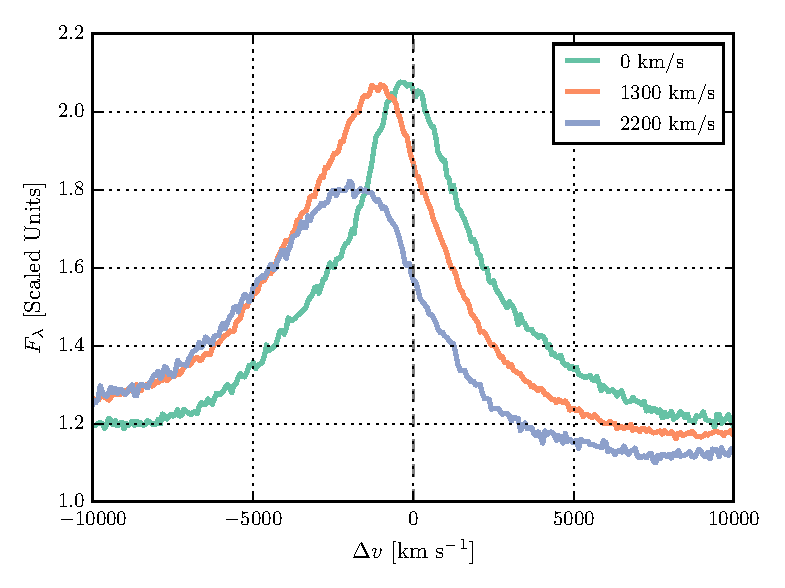
\includegraphics[width=0.9\linewidth]{figures/chapter03/civ_composites.pdf}
    \caption[{Composite spectra of the \ion{C}{IV}-emission line as a function of \ion{C}{IV} blueshift for SDSS DR7 quasars.}]{Composite spectra of the \ion{C}{IV}-emission line as a function of \ion{C}{IV} blueshift for SDSS DR7 quasars. Quasars classified as BALs, or possessing strong associated absorbers have been excluded, and the composite-spectra shown are derived using an arithmetic mean of a minimum of 200 spectra at each blueshift. Virtually the entire \ion{C}{IV}-profile appears to shift blueward and the change in line shape is not simply an enhancement of flux in the blue wing of a still identifiable symmetric component. In order of increasing \ion{C}{IV} blueshift, the composite spectra have FWHM 4870, 5610, and 6770 \kms\, and EW 33.1, 31.6, and 28.8 \AA.}
    \label{fig:civ_composites}
\end{figure}

Excess emission-line flux in the blue wing of the \ion{C}{IV} emission increases commonly employed measures of the line-width, notably the full-width at half maximum (FWHM) and the line dispersion ($\sigma$). 
In general, researchers studying quasar demographics at high-redshift adopt estimates of BH masses based on the width of \ion{C}{IV}-emission, without reference to the blueshift of the \ion{C}{IV}-emission \citep[e.g.][]{vestergaard04,kollmeier06,gavignaud08,vestergaard08,vestergaard09,kelly10,kelly13}. 
Figure~\ref{fig:civ_composites} shows the shape of the \ion{C}{IV}-emission in composite spectra constructed from SDSS DR7 quasars as a function of \ion{C}{IV} blueshift. 
The profiles show how, at large values of blueshift ($\gtrsim$2000\kms) the \ion{C}{IV}-profile is displaced to the blue by amounts comparable to the FWHM of the profile.
This indicates that non-virial motions, very likely due to outflows, are having a significant effect on the observed \ion{C}{IV} emission velocity profile \citep[e.g.][]{gaskell82,baskin05,sulentic07,richards11,wang13}. 
At fixed emission-line EW, virtually the entire \ion{C}{IV}-profile appears to shift blueward and the change in line shape is not simply an enhancement of flux in the blue wing of a still identifiable symmetric component. 
While gravity almost certainly plays a key role, determining the escape velocity for out-flowing material for example, it is clear that the virial assumption, on which single-epoch BH-mass measurements are predicated, is not straightforwardly applicable for the \ion{C}{IV}-emission line in quasars exhibiting large blueshifts. 
As a consequence, BH-masses derived from \ion{C}{IV} emission line velocity-widths are systematically biased compared to masses from the Balmer lines \citep[e.g.][]{shen08,shen12,coatman16}. 

As highlighted by \citet{richards11}, the sample of reverberation mapped quasars includes a restricted range of the \ion{C}{IV} emission line shapes seen in the quasar population. 
In particular, the reverberation mapped objects generally possess high \ion{C}{IV} equivalent widths and low \ion{C}{IV}-blueshifts. 
Nevertheless, the derived scaling relations based on the reverberation-mapped sample are regularly applied to the quasar population with low \ion{C}{IV} EWs and/or large \ion{C}{IV}-blueshifts, where any non-virial outflow-related contribution to the dynamics is significant. 

In recent literature, attempts have been made to minimise the influence of the systematic non-virial contribution to the \ion{C}{IV} emission on estimates of the BH mass. 
Strategies include (i) significantly reducing the dependence of the derived masses on the emission-line velocity width (e.g. from the $V^2$ dependence predicted assuming a virialized broad line region to just $V^{0.56}$ in \citealt{park13}; see also \citealt{shen12}), (ii) adopting a measure of emission-line velocity-width that is relatively insensitive to changes in the core of the emission-line profile \citep[e.g.][]{denney13} and (iii) estimating the amplitude of the non-virial contribution to the \ion{C}{IV} emission-line via comparison with other ultraviolet emission lines (e.g. \ion{Si}{IV}+\ion{O}{IV}$\lambda$1400 in \citealt{runnoe13} and \citealt{brotherton15}).
The increased number of quasars with high-quality spectra that cover both the observed-frame optical (where the redshifted \ion{C}{IV} appears) and near-infrared (where \hb and \ha lie) enables us to take a rather different approach in this chapter.
We will use properties of the \ion{C}{IV} emission line itself to reduce, or even remove, the systematic bias in the BH-mass estimates. 
Specifically, using the low-ionisation Balmer lines \ha and \hb as reliable proxies for the virial velocity, we will measure empirically the systematic bias in \ion{C}{IV}-based virial BH mass estimates as a function of the \ion{C}{IV} emission-line blueshift.

\section{Quasar Sample}

We have compiled a sample of 307 quasars at redshifts $1.5 < z < 4$ with both optical and near-infrared spectra.  
Reliable emission line properties were measured for 230 quasars (Section~\ref{sec:flagged_spectra}), with 164 possessing \ha line measurements and 144 \hb line measurements.  
This will allow us to directly compare virial BH mass estimates based on the \ion{C}{IV} line-width with estimates based on the line-widths of the low-ionisation Balmer lines \ha and \hbns.  
The sample is considerably larger than previous studies of the rest-frame optical spectra of high-$z$ quasars \citep[e.g.][]{shen12}. 
As we demonstrate in Section~\ref{sec:effectiveness}, the quasars have \ion{C}{IV} blueshifts of up to $\sim$5000\kms, and span the full range observed in the population. 

\subsection{Spectroscopic data}

The near-infrared data has been described in Chapter~\ref{ch:nirsample} and the telescopes/spectrographs used are summarised in Table~\ref{tab:specnums_ch3}. 
Corresponding optical spectroscopy was obtained from the SDSS (70 quasars), BOSS (126 quasars) and Hamburg/ESO surveys (15 quasars), and with VLT/UVES (11 quasars) and VLT/XSHOOTER (8 quasars). 
Many of the quasars in the SDSS DR$7$ catalogue have been re-observed as part of BOSS.
As the BOSS-spectra typically have higher S/N than the SDSS DR$7$ spectra, we have used the BOSS spectra when available.
Once more, further details are provided in Chapter~\ref{ch:nirsample}. 
We have sub-divided our sample into two overlapping groups: quasars with reliable \ha line measurements (the `\ha sample') and quasars with reliable \hb measurements (the `\hb sample').

\begin{table*}
  \small
  \centering
  \caption{The numbers of quasars with reliable \ha and \hb line measurements, and the spectrographs and telescopes used to obtain the near-infrared spectra}
  \label{tab:specnums_ch3}
  \centering
    \begin{tabular}{cccc} 
    \hline
    Spectrograph & Telescope & \ha Sample & \hb Sample \\
    \hline
    FIRE       & MAGELLAN & 18 & 19 \\
    GNIRS      & GEMINI-N & 22 & 17 \\
    ISAAC      & VLT      & 0  & 4 \\
    LIRIS      & WHT      & 15 & 0 \\
    NIRI       & GEMINI-N & 0  & 12 \\
    SINFONI    & VLT      & 2  & 25 \\
    SOFI       & NTT      & 47 & 23 \\
    TRIPLESPEC & ARC-3.5m & 33 & 20 \\
    TRIPLESPEC & P200     & 23 & 19 \\
    XSHOOTER   & VLT      & 4  & 7 \\
    \hline
    \multicolumn{2}{c}{Total} & 164 & 144 \\
    \hline
    \end{tabular}
\end{table*}

\section{Spectral Measurements}
\label{sec:spec_measures}

Conventionally, single-epoch virial estimates of the BH mass are a function of the line-of-sight velocity width of a broad emission line and the quasar luminosity. 
The velocity width is a proxy for the virial velocity in the broad line region (BLR) and, as revealed in reverberation-mapping studies, the luminosity is a proxy for the typical size of the BLR \citep[the $R-L$ relation; e.g.][]{kaspi00,kaspi07}. 
Most reverberation mapping campaigns have employed \hb time-lags and velocity widths, but the line-widths of \ha and \ion{Mg}{II}$\lambda$2800 have been shown to yield consistent BH masses \citep[e.g.][]{mclure02,greene05b,onken08,shen08,wang09,rafiee11,mejia-restrepo16}. 
In Section~\ref{sec:hahbcomparison} we verify that the \ha and \hb line-widths yield consistent BH for the 99 quasars in our sample with measurements of both.     

In our work, a robust measure of the \ion{C}{IV} emission-line `blueshift' provides the basis for the corrected \ion{C}{IV} velocity-width measurements, and hence BH masses.
The effectiveness of the scheme is validated via a direct comparison of the \ion{C}{IV} velocity-widths to the Balmer emission velocity-widths in the same quasars. 
Our process is as follows. 
First, an accurate measure of the quasar's systemic redshift is required, for which we adopt the centre of the Balmer emission, where the centre, $\lambda_{\mathrm half}$, is the wavelength that bisects the cumulative total flux. 
Balmer emission centroids are available for all quasars in the catalogue but we verify that the measure is relatively unbiased through a comparison of the centroids to the wavelengths of the peak of the narrow [\ion{O}{III}]\ll4960,5008 doublet for the subset of spectra where both are available (Section~\ref{sec:zsys}). 
Second, the blueshift of the \ion{C}{IV} emission line is determined. 
Again, we adopt the line centroid to provide a robust measure of the \ion{C}{IV} emission blueshift.
The blueshift (in \kms) is defined as $c\times$(1549.48-$\lambda_{half}$)/1549.48 where $c$ is the velocity of light and 1549.48\,\AA \ is the rest-frame wavelength for the \ion{C}{IV} doublet\footnote{The adopted \ion{C}{IV} rest-frame wavelength assumes an optically thick BLR, in which case the contribution from each component is equal. Adopting a 2:1 ratio (appropriate for an optically thin BLR) changes the blueshifts by $\sim$80\kms.}. 
Positive blueshift values indicate an excess of emitting material moving towards the observer and hence out-flowing from the quasar. 

Emission-line velocity widths are derived from the full-width-at-half-maximum (FWHM) of the lines but we also compute the line dispersion (calculated from the flux-weighted second moment of the velocity distribution) as some authors have claimed this provides a better estimate of the virial velocity \citep{denney13}. 

To minimise the impact of the finite S/N of the quasar spectra and the presence of absorption features superposed on the broad emission lines we first fit a parametric model to the continuum and the emission lines. 
The particular form of the model parametrizations is not important and the fits are used only to provide robust line parameters, such as the centroid $\lambda_{\mathrm half}$, and FWHM, which are measured non-parameterically from the best-fitting model. 
The models used and the fitting procedure are described below. 
The issues involved in deriving parameters for broad emission lines from spectra of modest S/N -- for example, subtraction of narrow line emission, subtraction of \ion{Fe}{II} emission -- have been covered comprehensively by other authors \citep[e.g.][]{shen11,shen12,denney13,shen16a} and, as far as possible, we follow standard procedures described in the literature. 

\subsection{\ion{C}{IV}}
\label{sec:civ}

We first define a power-law continuum, $f(\lambda) \propto \lambda^{-\alpha}$, with the slope, $\alpha$, determined using the median values of the flux in two continuum windows at 1445-1465 and 1700-1705\AA. 
The continuum emission is subtracted from the spectra, which is then transformed from wavelength units into units of velocity relative to the rest-frame line-transition wavelength for the \ion{C}{IV} doublet.
The parametric model is ordinarily fit within the wavelength interval 1500-1600\AA\, (corresponding to approximately $\pm 10\,000$ \kms\, from the rest-frame transition wavelength), a recipe that is commonly adopted \citep[e.g.][]{denney13}. 
The line-window was extended if more than 5\,per cent of the total flux in the profile was present blueward of the short wavelength limit. 
Narrow absorption features, which are frequently found superimposed on \ion{C}{IV} emission, were masked out during the fit. 

The \ion{C}{IV} emission was fit with sixth-order Gauss-Hermite (GH) polynomials, using the normalisation of \citet{marel93} and the functional forms of \citet{cappellari02}. 
We allowed up to six components, but in many cases a lower order was sufficient (40 and 45 per cent were fit with second- and fourth-order GH polynomials respectively).
GH polynomials were chosen because they are flexible enough to model the often very asymmetric \ion{C}{IV} line profile. 
The flip-side of this flexibility, however, is that the model has a tendency to over-fit when spectra possess low S/N. 
The fits were therefore carefully checked visually and the number of components reduced if over-fitting was evident.

We find that using the commonly employed three-Gaussian component model, rather than the GH polynomials, resulted in only marginal differences in the line parameters. 
Our best-fit parameters are also in good agreement with \citet{shen11}, who employ a multi-Gaussian parametrization. 
In Fig.~\ref{fig:shen_comparison_civ} we compare our measurements of the \ion{C}{IV} FWHM from the 71 SDSS DR7 spectra in our sample with the measurements published in \citet{shen11}. 
There is a very strong agreement between our measurements, with a scatter of 0.05 dex (200\kms). 

\begin{figure}
    \centering 
    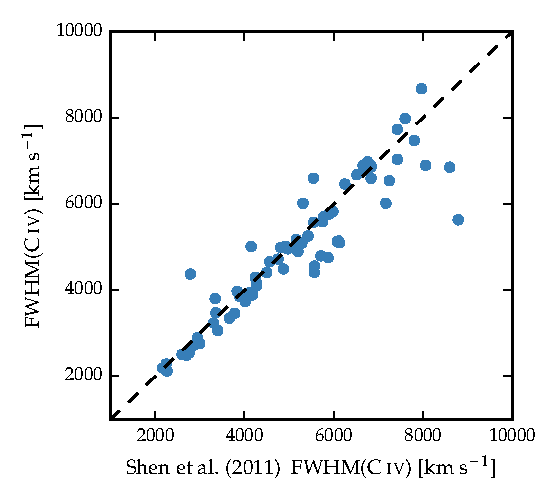
\includegraphics[width=0.8\linewidth]{figures/chapter03/shen_comparison_civ.pdf} 
    \caption{Demonstration of the effectiveness of our line parameter estimation scheme via a comparison of the \ion{C}{IV} FWHM with \citet{shen11}.} 
    \label{fig:shen_comparison_civ}
\end{figure}

\subsection{\ha}
\label{sec:ha}


A power-law continuum is fit using two continuum windows at 6000-6250 and 6800-7000\,\AA. 
The continuum-subtracted flux is then fit in the wavelength interval 6400-6800\,\AA. 
We adopt a rest-frame transition wavelength of 6564.89\,\AA\, to transform wavelengths into equivalent Doppler velocities. 
The broad component of \ha is fit using one or two Gaussians, constrained to have a minimum FWHM of 1200\kms. When two Gaussians are used, the velocity centroids are constrained to be the same.

The emission-line profiles of both \hb and \ha frequently include a significant narrow component from the physically more extended narrow line region (NLR). 
Additional Gaussian components were included in our parametric model to fit the narrow component of \ha as well as [\ion{N}{II}]\ll6548,6584 and [\ion{S}{II}]\ll6717,6731.
This resulted in a better fit to the observed flux in 50\, per cent of cases. 
We impose a 1200\kms upper limit on the FWHM of all narrow lines and the amplitudes of all components must be non-negative.
The relative flux ratio of the two [\ion{N}{II}] components is also fixed at the expected value of 2.96.
In 70\, per cent of the spectra the [\ion{O}{III}]\ll4960,5008 doublet is detected at moderate S/N in the \hb region. 
In these cases the peak of the [\ion{O}{III}] is used to fix the velocity offsets and the FWHMs of the narrow line components in the \ha region.  
For spectra where the [\ion{O}{III}] doublet does not constrain the velocity and FWHM accurately, the narrow emission in the \ha and \hb regions are fitted independently but, for each region, the individual narrow-line velocity offsets and the FWHMs are constrained to be identical. 
In these objects the narrow line contribution is generally weak, and so does not have a large effect on the line parameters we measure for the broad component.   

The model described above is very similar to the one described in \citet{shen12} and \citet{shen11}, the only major differences being that we do not fit the \ha and \hb emission regions simultaneously and we fix the centroids of the Gaussian components used to fit the broad emission.
In Fig.~\ref{fig:shen_comparison_ha} we plot our \ha FWHM measurements against the measurements published in \citet{shen12}, for 51 quasars in common to both samples.
There is a strong correlation and a scatter of just 0.07 dex. 

\begin{figure}
    \centering 
    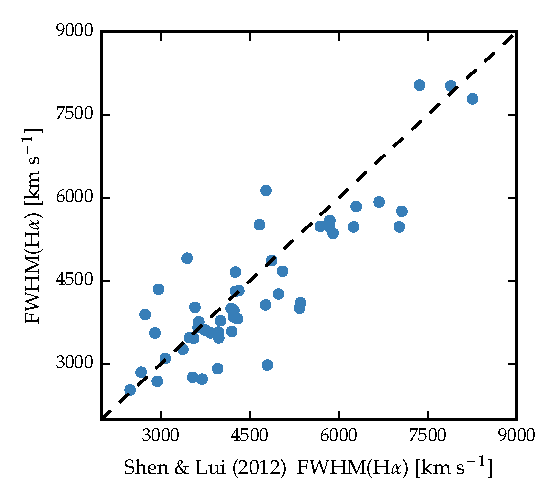
\includegraphics[width=0.8\linewidth]{figures/chapter03/shen_comparison_ha.pdf} 
    \caption{Demonstration of the effectiveness of our line parameter estimation scheme via a comparison of the \ha FWHM with \citet{shen12}.} 
    \label{fig:shen_comparison_ha}
\end{figure}

\subsection{\hb and [\ion{O}{III}]}
\label{sec:hb}

Emission from optical \ion{Fe}{II} is generally strong in the vicinity of \hbns.
We therefore fit a combination of a power-law continuum and an optical \ion{Fe}{II} template -- taken from \citet{boroson92} -- to two windows at 4435-4700 and 5100-5535\,\AA. 
The \ion{Fe}{II} template is convolved with a Gaussian, and the width of this Gaussian, along with the normalisation and velocity offset of the \ion{Fe}{II} template, are free variables in the pseudo-continuum fit.
We use the same model to fit the broad and narrow components of \hb as was used with \hans. 
Each line in the [\ion{O}{III}] doublet is fit with two Gaussians, to model both the systemic and any outflow contributions. 
The peak flux ratio of the [\ion{O}{III}] 4960\,\AA\, and 5008\AA\, lines is fixed at 1:3. 
As for the fit to the narrow lines in the spectral region around \hans, the width and velocity offsets of all the narrow components are set to be equal, and an upper limit of 1200\kms is placed on the FWHM. 

The parametric model we fit to the \hbns/[\ion{O}{III}] emission region was very similar to the model employed by \citet{shen16a}. 
In Fig.~\ref{fig:shen_comparison_hb} we plot our \hb FWHM measurements against the measurements published in \citet{shen16a}, for 39 quasars in common to both samples. 
As expected, we observe a very tight correlation, with a scatter of 0.04 dex. 

\begin{figure}
    \centering 
    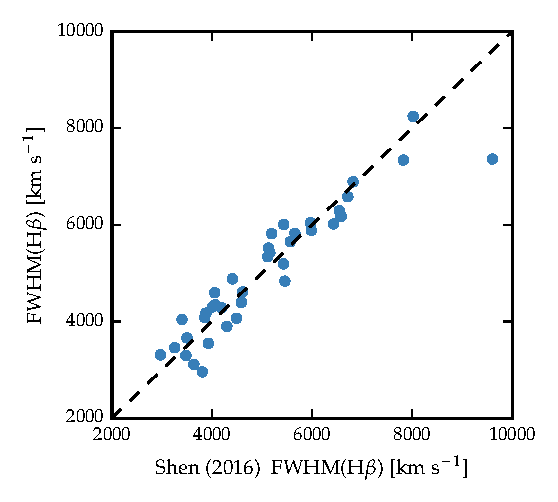
\includegraphics[width=0.8\linewidth]{figures/chapter03/shen_comparison_hb.pdf} 
    \caption{Demonstration of the effectiveness of our line parameter estimation scheme via a comparison of the \hb FWHM with \citet{shen16a}.} 
    \label{fig:shen_comparison_hb}
\end{figure}

\subsection{Fitting procedure}

Model parameters were derived using a standard variance-weighted least-squares minimisation procedure employing the Levenberg-Marquardt algorithm. 
Prior to the fit, the spectra were inspected visually and regions significantly affected by absorption or of low S/N were masked out.

In Fig.~\ref{fig:examplegrid} we present our parametric fits to the \ion{C}{IV}, \ha and \hb emission lines in a handful of quasars, which have been chosen to illustrate the range of spectrum S/N and line shapes in the sample.  
The Doppler velocities have been shifted so that the \ha emission line centroid is at 0\,\kms. 
The $y$-axes of the data-minus-model residual plots have been scaled by the spectrum flux errors.
The mean reduced chi-squared values in our \hans, \hb and \ion{C}{IV} fits are 1.69, 1.62, and 1.77 respectively and, in general, there are no strong features observable in the spectrum minus model residuals. 
The only significant features seen in the residual \ion{C}{IV} spectra correspond to the location of narrow absorption lines which were excluded in the fitting procedure.

Table~\ref{tab:bhm-specmeasure} includes the line parameters of our best-fitting model for each line.

\begin{table*}
  \small 
  \centering
  \caption{The format of the table containing the emission line properties from our parametric model fits. The table is available in machine-readable form in the online version of \citet{coatman17}.}
  \label{tab:bhm-specmeasure}
   \begin{tabular}{ccc} 
    \hline
    & Units & Description \\ 
    \hline
    NAME & & Catalogue name \\
    FWHM\_BROAD\_HA & \kms & FWHM of broad \ha line \\ 
    FWHM\_BROAD\_HA\_ERR & \kms & \\
    SIGMA\_BROAD\_HA & \kms & Dispersion of broad \ha line\\
    SIGMA\_BROAD\_HA\_ERR & \kms & \\
    Z\_BROAD\_HA & & Redshift from broad \ha line\\
    FWHM\_BROAD\_HB & \kms & FWHM of broad \hb line \\
    FWHM\_BROAD\_HB\_ERR & \kms & \\
    SIGMA\_BROAD\_HB & \kms & Dispersion of broad \hb line \\
    SIGMA\_BROAD\_HB\_ERR & \kms & \\
    Z\_BROAD\_HB & & Redshift from broad \hb line\\
    FWHM\_CIV & \kms & FWHM of \ion{C}{IV} doublet \\
    FWHM\_CIV\_ERR & \kms & \\
    SIGMA\_CIV & \kms & Dispersion of \ion{C}{IV} doublet \\
    SIGMA\_CIV\_ERR & \kms & \\
    BLUESHIFT\_CIV\_HA & \kms & Blueshift of \ion{C}{IV} relative to \hans \\
    BLUESHIFT\_CIV\_HA\_ERR & \kms & \\
    BLUESHIFT\_CIV\_HB & \kms & Blueshift of \ion{C}{IV} relative to \hbns \\
    BLUESHIFT\_CIV\_HB\_ERR & \kms & \\
    LOGL5100 & \ergs & Luminosity at 5100\AA \\
    LOGL1350 & \ergs & Luminosity at 1350\AA\\
    \hline
    \end{tabular}
\end{table*}

\begin{figure}
    \centering
    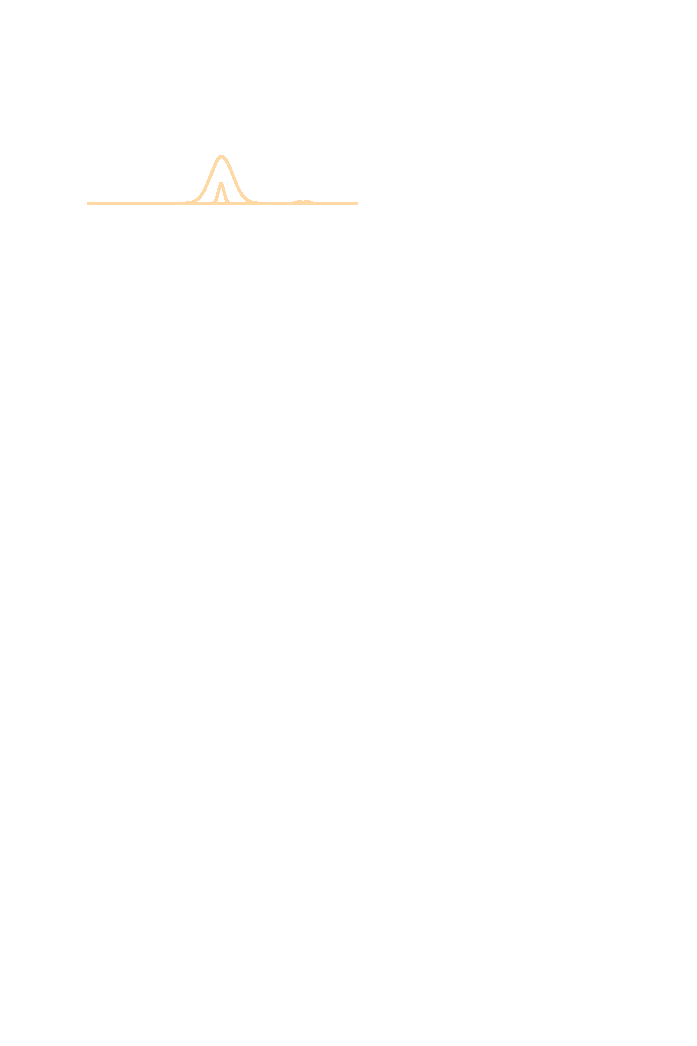
\includegraphics[width=\linewidth]{figures/chapter03/example_spectrum_grid.pdf} 
    \caption[{Model fits to continuum-subtracted \hans, \hbns, and \ion{C}{IV} emission in four quasars, chosen to represent the range of S/N and line shapes present in the catalogue.}]{Model fits to continuum-subtracted \hans, \hbns, and \ion{C}{IV} emission in four quasars, chosen to represent the range of S/N (indicated in the figure and given per 150\kms\, pixel in the continuum) and line shapes present in the catalogue. The data is shown in grey, the best-fitting parametric model in black, and the individual model components in orange. The centroid of the broad \ha emission is used to set the redshift, and $\Delta{v}$ is the velocity shift from the line rest-frame transition wavelength. Below each fit we plot the data minus model residuals, scaled by the errors on the fluxes.} 
    \label{fig:examplegrid}
\end{figure}


\subsection{Spectra removed from sample}
\label{sec:flagged_spectra}

\begin{table}
  \centering
  \caption{The number of spectra removed from our sample by the cuts described in Section~\ref{sec:flagged_spectra}.}
  \label{tab:flagged_spectra}
    \begin{tabular}{cccc}
    \hline
    & & \ha sample & \hb sample \\ 
    \hline
    \multicolumn{2}{c}{Total} & 194 & 279 \\
    \hline
    \hans/\hbns & Wavelength & 6 & 27 \\
    & S/N & 8 & 83 \\
    \hline
    \ion{C}{IV} & Wavelength & 6 & 5 \\
    & S/N & 4 & 12 \\
    & Absorption & 6 & 8 \\
    \hline
    \multicolumn{2}{c}{Total remaining} & 164 & 144 \\
    \hline
    \end{tabular}
\end{table}


Through visual inspection we flagged and discarded the spectra of quasars for which reliable emission line parameters could not be obtained.

First, we flagged emission lines in spectra that possessed insufficient S/N. 
A single minimum S/N threshold was not entirely effective and, instead, spectra were flagged when it was judged conservatively that no meaningful constraints could be placed on the velocity centroid and/or width of the emission-line. 

Second, we flagged emission lines where significant regions of the continuum and/or emission line fell outside of the wavelength coverage of the spectra. 
Reliable continuum definition and subtraction is not straightforward for emission lines so affected. 

Third, we flagged \ion{C}{IV} emission lines because of strong, narrow absorption close to the peak of the line where reliable interpolation across the absorption, using our parametric model, was not possible. 

The number of spectra that are removed by each cut is given in Table~\ref{tab:flagged_spectra} and the distribution in redshift and luminosity is shown in Fig.~\ref{fig:flagged_spectra}. 
Unsurprisingly, there is a preferential removal of intrinsically faint quasars, whose spectra can be of poorer S/N, and a loss of quasars at redshifts $z\sim2.6$ where the \ha emission falls at the edge of the $K$-band.
\hb is much weaker than \hans, and the \hb spectra are generally of lower S/N. 
As a result, the fraction of \hb spectra that are flagged -- 39 per cent -- is particularly high.   

\begin{figure}[h!]
    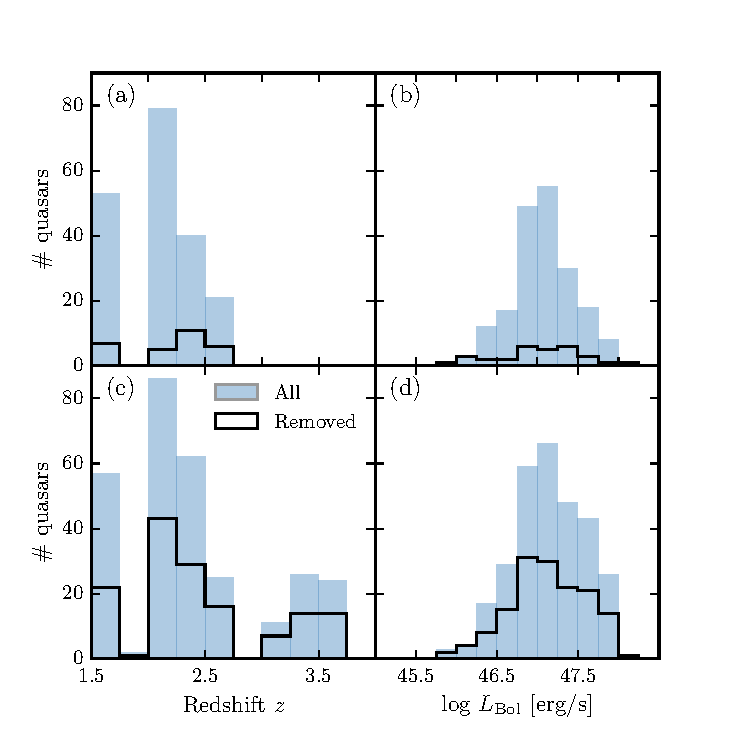
\includegraphics[width=\textwidth]{figures/chapter03/flagged_spectra.pdf} 
    \caption{The redshift and luminosity distributions of the spectra removed from our \hans/\ion{C}{IV} (a, b) and \hbns/\ion{C}{IV} (c, d) samples.} 
    \label{fig:flagged_spectra}
\end{figure}

\subsection{Emission-line parameter uncertainties}
\label{sec:ch3_param_errors}

The 1$\sigma$ error bars calculated from the covariance matrix in least-squares minimisation will underestimate the true uncertainties on the line parameters, since they do not account for systematic errors such as the significant uncertainty introduced in the continuum subtraction procedure.  
To calculate more realistic uncertainties on our fitted variables we employed a Monte Carlo approach. 
One thousand artificial spectra were synthesised, with the flux at each wavelength drawn from a Normal distribution (mean equal to the measured flux and standard deviation equal to the known error).
Our emission-line fitting recipe was then implemented on each of these mock spectra. 
The uncertainty in each parameter is given by the spread in the best-fitting values from the one thousand realisations of the fitting routine. 
In some cases the standard deviation of the parameter distribution was biased by extreme values caused by bad fits\footnote{In the analysis of the real spectra such fits are identified via visual inspection.}. 
We therefore chose to measure the spread in the parameter distribution by fitting a composite model with two Gaussian components -- one to model uncertainty in the parameter and the other any possible outlier component. 
The uncertainty in each line parameter was then taken to be the width of the narrower Gaussian. 
The uncertainties on all derived quantities, such as the BH mass, are propagated through by assuming that the uncertainties are uncorrelated and independent. 

\subsection{Contemporaneity of spectra}

The epochs of the near-infrared and optical spectra can differ by many years.
For example, the NTT SOFI spectra were taken $\sim$14 years after the SDSS spectra, and the VLT SINFONI spectra 20 years or more after the Hamburg/ESO observations\footnote{Time differences in the quasar rest-frame are reduced by a factor of ($1 + z$).}.
If the broad emission line profiles varied significantly on these time-scales the relation between the \ion{C}{IV} and Balmer line-width measurements could be blurred. 

Cases do exist of dramatic changes in quasar spectra over short time-scales, but this phenomenon is rare \citep{macleod16}. 
In our spectroscopic catalogue there are 112 SDSS DR7 quasars which are re-observed in BOSS and included in the DR12 quasar catalogue. 
The mean time elapsed between the two sets of observations is $\sim$8 years. 
The root-mean-square difference in the \ion{C}{IV} FWHM measured from the BOSS and SDSS spectra is a modest $\simeq$500\kms. 
Differences in the S/N of the spectra will make a substantial contribution and the scatter due to true variations in the \ion{C}{IV} velocity-width will be significantly smaller than 500\kms. 
We conclude therefore that any intrinsic changes with time do not materially affect the emission line measurements.

\subsection{Quasar monochromatic luminosity}

Computing virial BH masses also requires the quasar luminosity in an emission-line free region of the continuum adjacent to the broad line being used. 
The luminosity is used as a proxy for the size of the BLR. 
The monochromatic continuum flux is generally measured at 1350\,\AA\ for \ion{C}{IV} and 5100\,\AA\, for \ha and \hbns. 
The calculation of these luminosities is described in Chapter~\ref{ch:nirsample}. 

As described in Chapter~\ref{ch:nirsample}, we estimate the uncertainties on the monochromatic luminosities to be $\sim$0.3 dex. 
Given that the luminosity enters into the calculation of BH-mass only as the square-root, the uncertainty on the luminosities does not make a large contribution to the uncertainties in the BH mass estimates.  

\subsection{Characterising the emission-line widths}
\label{sub:charemprof}

\begin{figure}
    \centering 
    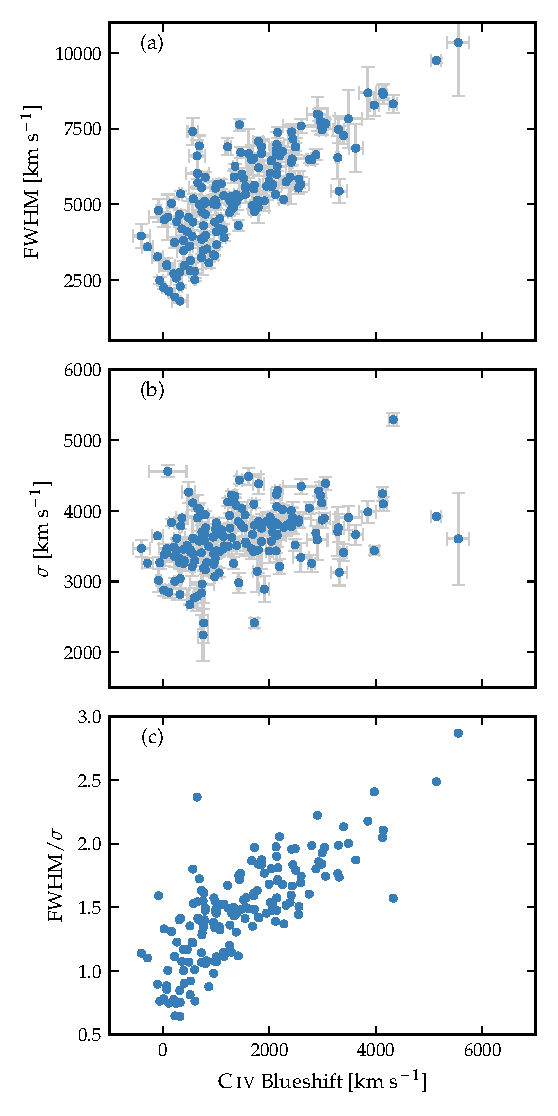
\includegraphics[width=0.8\linewidth]{figures/chapter03/civ_comparisons_paper2.pdf} 
    \caption{The FWHM, dispersion ($\sigma$) and shape (FWHM/$\sigma$) of \ion{C}{IV} as a function of the \ion{C}{IV} blueshift.}
    \label{fig:line_comparison_civ}
\end{figure} 

There has been a considerable degree of attention paid to the effectiveness of different velocity-width measures of the \ion{C}{IV}-emission; specifically, the line FWHM and the dispersion, $\sigma$, derived from the second-moment velocity \citep[e.g.][]{assef11, denney13}.
The FWHM and line dispersion trace different parts of the broad line velocity field, with the FWHM relatively more sensitive to any low-velocity core present and the line dispersion relatively more sensitive to the high velocity wings. 
In practice, the line dispersion is almost certainly a more robust velocity indicator when the assumptions underlying the virial-origin of the emission-line velocity width are true and the spectral S/N and resolution are adequate.
This was demonstrated by \citet{denney13} for a sample of quasars possessing a significantly smaller range in \ion{C}{IV}-blueshift than investigated here.

In reality, however, as highlighted by \citet{denney12}, contributions to the \ion{C}{IV}-emission line profile from gas where virial motions do not dominate can be significant. 
Looking to the future, the results of the new reverberation-mapping projects \citep{shen15, kingoz15} will show what fraction of the \ion{C}{IV}-emission line, as a function of velocity, does reverberate for quasars with an extended range of \ion{C}{IV}-emission shapes. 
The derivation of quantitative corrections to transform velocity-width measures from single-epoch to reverberation-only line profiles should then be possible. 

As such information is not yet available, there is a strong rationale for investigating whether the systematic changes in the \ion{C}{IV}-emission line profile can be used to improve the single-epoch BH-mass estimates derived using the \ion{C}{IV} line. 
In Fig.~\ref{fig:line_comparison_civ} we show how the \ion{C}{IV} FWHM, line dispersion, $\sigma$, and line shape, FWHM/$\sigma$, vary as a function of the blueshift. 
The \ion{C}{IV} FWHM is correlated with the blueshift, with the median FWHM of quasars with the largest blueshifts a factor of 2-3 higher than quasars with only moderate blueshifts.
The dispersion, however, does not show a similarly strong systematic variation. 

Without knowledge of the \ion{C}{IV}-blueshifts, the dynamic range present in the FWHM and line dispersion measurements accords with the expectations from the study of \citet{denney13}; the factor of $\simeq$4 spread in the FWHM measurements indicating greater sensitivity to the emission-line profile shape than is the case for the dispersion, which varies by a factor of only $\lesssim$2.
Adopting a value of 1200\,\kms\, to define `low' and `high' blueshift, the median \ion{C}{IV}-emission dispersion for the low and high-blueshift samples differ by only 10 per cent. 
It follows, therefore, that while the dispersion provides a relatively line-profile independent measure of the velocity width for quasars where the underlying assumption regarding the virial-origin of the velocity width applies, quasars where the assumption is not true can be assigned apparently normal velocity-widths and hence potentially incorrect BH-masses. 

To emphasise this point, in Fig.~\ref{fig:civ_comparison} we overlay the \ion{C}{IV} line profiles of SDSSJ1236+1129 and SDSSJ1525+2928, whose dispersions are indistinguishable (4168$\pm$271 and 4303$\pm$128\,\kms respectively). 
Notwithstanding the very similar dispersion values, the emission-line velocity fields differ dramatically and, therefore, the dispersion values cannot be measuring accurately the virial-induced velocity spread of the \ion{C}{IV} emission in both quasars.

The analysis here, building on earlier work \citep[including][]{shen12, sulentic07}, confirms a link between \ion{C}{IV} emission-line shape and blueshift, raising the prospect of developing a blueshift-dependent correction to single-epoch BH-mass estimates based on the \ion{C}{IV} line. 
Expressed in another way, we are interested in testing if the significant systematic change in line shape as a function of \ion{C}{IV} blueshift can be used to provide improved single-epoch BH-masses from the \ion{C}{IV} emission line.  
The tightness of the correlation we observe between the \ion{C}{IV} FWHM and blueshift implies that such an approach may be more effective than using the \ion{C}{IV} emission-line velocity dispersion without reference to blueshifts.
A further practical advantage is that, given the typical S/N of current survey-quality spectra, virial BH mass estimates for high-redshift quasars are usually based on the FWHM rather than the dispersion \citep[e.g.][]{shen11}, which, being strongly affected by the continuum placement, is often found to be difficult to measure robustly \citep[e.g.][]{mejia-restrepo16}. 

\begin{figure}
    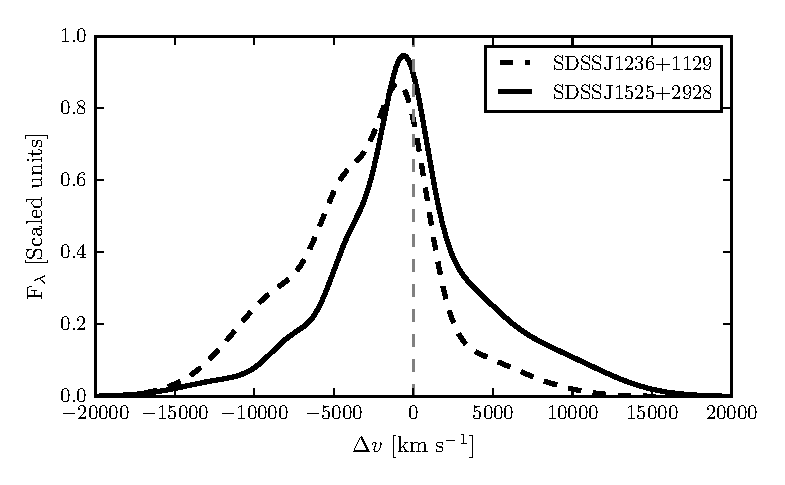
\includegraphics[width=\linewidth]{figures/chapter02/civ_comparison.pdf} 
    \caption[{Comparison of the \ion{C}{IV} line profiles of SDSSJ1236+1129 and SDSSJ1525+0426.}]{Comparison of the \ion{C}{IV} line profiles of SDSSJ1236+1129 and SDSSJ1525+0426. Notwithstanding the essentially identical dispersion values, the emission-line velocity fields differ dramatically and, therefore, the dispersion values cannot be measuring accurately the virial-induced velocity spread of the \ion{C}{IV} emission in both quasars. }
    \label{fig:civ_comparison}
\end{figure}

\section{An empirical correction to \ion{C}{IV}-based virial BH-mass estimates}

\subsection{\hans/\hb FWHM comparison}
\label{sec:hahbcomparison}

BH-mass calibrations which use the width of the broad \hb emission line as a proxy for the virial velocity are widely regarded as the most reliable, since most reverberation mapping employs the \hb line and the $R-L$ relation has been established using \hbns.
When \hb is not available, \ha has been shown to be a reliable substitute \citep[e.g.][]{greene05b,shen11,shen12}. 

\begin{figure}
    \centering 
    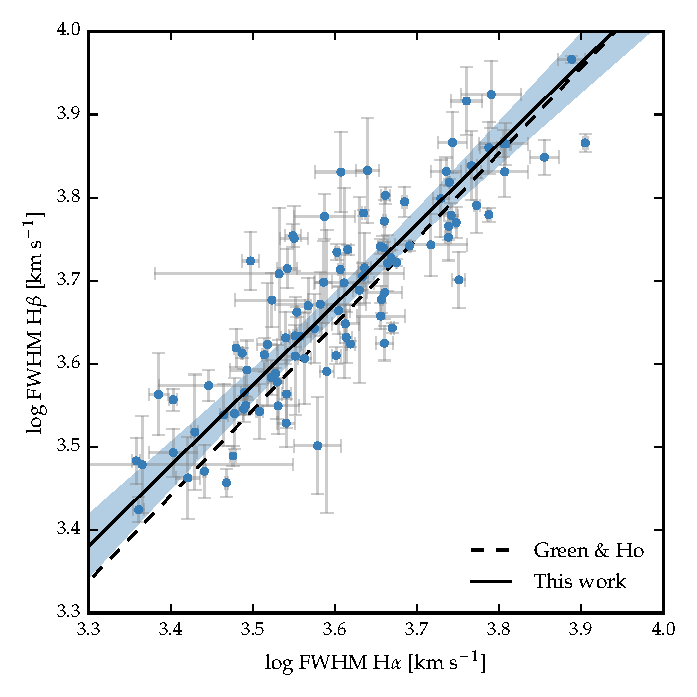
\includegraphics[width=0.8\columnwidth]{figures/chapter03/ha_hb_width_comparison.pdf} 
    \caption[{Comparison of \ha and \hb FWHM measurements for 99 quasars.}]{Comparison of \ha and \hb FWHM measurements for 99 quasars. The solid line is our best-fitting power-law model, and the blue-shaded region shows the 2-$\sigma$ uncertainties on the model parameters. The dashed line is the relation found by \citet{greene05b} using a sample of $z<0.35$ SDSS AGN.} 
    \label{fig:hahbcomp}
\end{figure}

In our sample, we have 99 quasars with reliable measurements of both \ha and \hb lines. 
The 99 objects include 21 quasars which were excluded from the main 308-object catalogue because the \ion{C}{IV} FWHM and/or blueshift could not be measured reliably. 
The line widths are compared in Fig.~\ref{fig:hahbcomp} and, as expected, a tight correlation is observed.  
\citet{greene05b}, using a sample of 162 quasars with high S/N SDSS spectra at $z < 0.35$, established the following relation between the \ha and \hb FWHMs

\begin{equation}
  \mathrm{FWHM}(\mathrm{H}\beta) = \left( 1.07 \pm 0.07 \right) \times 10^3 \left( \frac{ \mathrm{FWHM}(\mathrm{H}\alpha) }{10^3 ~\mathrm{km}~\mathrm{s}^{-1} } \right)^{(1.03 \pm 0.03)}
\end{equation}

The relation is shown as the dashed line in Fig.~\ref{fig:hahbcomp}.
The root-mean-square scatter about this relation is 0.07\,dex, compared to the $\sim$0.1\,dex found by \citet{greene05b}. 
However, we find a systematic offset, in the sense that the \hb line-widths we measure are on average larger by 270\kms\, than predicted by the \citet{greene05b} relation. 
As our sample covers higher redshifts and luminosities than the sample in \citet{greene05b}, we derive a new relation between the \ha and \hb FWHMs.       

We assume a relation of the same form used by \citet{greene05b}, i.e. a simple power-law, and infer the model parameters by fitting a linear model (with slope $\alpha$ and intercept $\beta$) in log-log space.
The fit is performed within a Bayesian framework described by \citet{hogg10}. 
Each data point is treated as being drawn from a distribution function that is a convolution of the projection of the point's covariance tensor, of variance $\Sigma_i^2$, with a Gaussian of variance $V$ representing the intrinsic variance in the data.
The log-likelihood is then given by 

\begin{equation}
  {\mathrm ln} {\cal L} = - \sum_{i=1}^N \frac{1}{2} {\mathrm ln}\left[2\pi\left(\Sigma_i^2 + V\right)\right] - \sum_{i=1}^N \frac{\Delta_i^2}{2[\Sigma_i^2 + V]} 
\end{equation}

\noindent where $\Delta_i$ is the orthogonal displacement of each data point from the linear relationship. 
An advantage of this approach is that it allows a proper treatment of the measurement errors on both variables, which in this case are comparably large.
The model also makes the reasonable assumption that there is an intrinsic scatter in the relationship between the variables that is independent of the measurement errors.  
Following the suggestion by \citet{hogg10}, the linear model was parametrized in terms of ($\theta$,~$b_\bot$), where $\theta$ is the angle the line makes with the horizontal axis and $b_\bot$ is the perpendicular distance from the line to the origin.
Uniform priors were placed on these parameters, and the Jeffreys prior (the inverse variance) was placed on the intrinsic variance. 
The posterior distribution was sampled using a Markov Chain Monte Carlo (MCMC) method using the Python package {\tt emcee} \citep{foreman13}. 
 
The one- and two-dimensional posterior distributions are shown in Fig.~\ref{fig:ha_hb_mcmc_samples}. 
The solid line in Fig.~\ref{fig:hahbcomp} is the maximum likelihood solution

\begin{equation}
  \label{eq:ha2hb}
  \mathrm{FWHM}(\mathrm{H}\beta) = \left( 1.23 \pm 0.10 \right) \times 10^3 \left( \frac{\mathrm{FWHM}(\mathrm{H}\alpha)}{10^3 {\mathrm km\,s^{-1}}} \right)^{0.97 \pm 0.05}
\end{equation}

\noindent and the shaded region shows the 2$\sigma$ uncertainties on the model parameters.

As discussed above, our relation is displaced to slightly higher \hb FWHM than the \citet{greene05b} relation -- the offset is 210\kms\, for a quasar with \ha FWHM 4500\kms.  
We infer a power-law index that, although slightly shallower, is consistent with the \citet{greene05b} index within the quoted uncertainties. 
The intrinsic scatter in the data, $\sigma_I$, we infer from  the fit is 0.04 dex. 
This is smaller than the total scatter seen in Fig.~\ref{fig:hahbcomp} (0.06 dex), which suggests that measurement errors make a significant contribution to the total scatter in the relation. 

\begin{figure}[h!]
    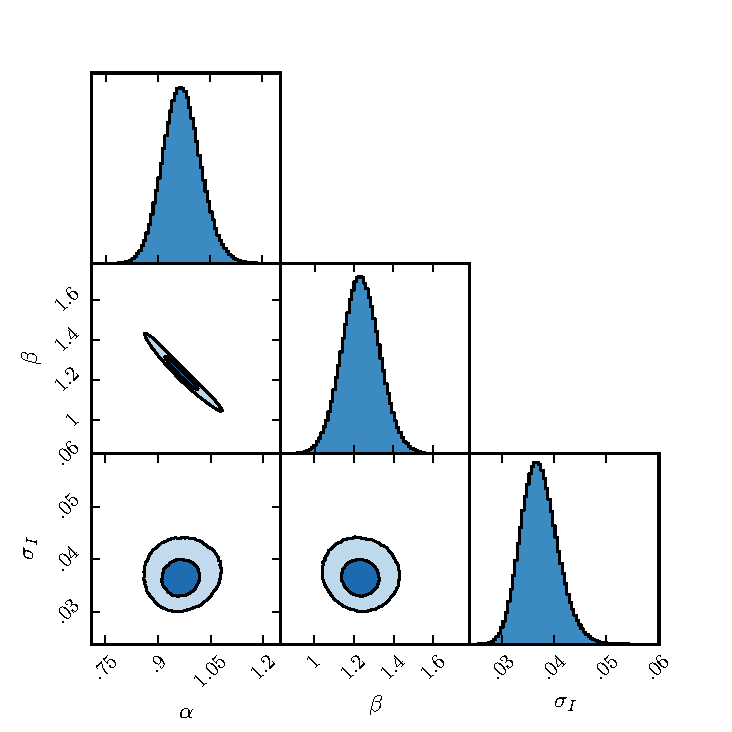
\includegraphics[width=\columnwidth]{figures/chapter03/ha_hb_mcmc_parameters.pdf} 
    \caption[{One- and two-dimensional projections of the MCMC sampling of the posterior distribution from the fit in Fig.~\ref{fig:hahbcomp}.}]{One- and two-dimensional projections of the MCMC sampling of the posterior distribution from the fit in Fig.~\ref{fig:hahbcomp}. $\alpha$ is the power-law index, $10^\beta$ is the normalisation, and $\sigma_I$ is the intrinsic scatter. In the two-dimensional projections, 1- and 2-$\sigma$ contours are shown.} 
    \label{fig:ha_hb_mcmc_samples}
\end{figure}

We constructed composite spectra of the \ha and \hb regions from 217 and 171 quasars respectively. 
Spectra were first de-redshifted to the quasar rest-frame, and then interpolated on to a common wavelength grid with a 1\AA\, resolution. 
The spectra were scaled by the mean flux in the interval 4700-5100\AA\, (\hbns) and 6400-6800\AA\, (\hans). 
The composite was then defined as the median flux from all of the normalised spectra in each wavelength bin. 
The \ha and \hb lines in the composite spectra are shown in Fig.~\ref{fig:balmer_composite}.
The cores of the two lines are very similar, but \hb has more flux in the wings of the line. 

For 19 of the 99 quasars with \hb and \ha emission profiles, one of the two Gaussians used to reproduce the \hb profiles has a FWHM greater than 20\,000\kms and a fractional contribution to the total \hb broad line flux of $>$0.3 \citep{marziani09,marziani13}.  
Such a broad component is not seen in the \ha profiles and the very broad \hbns-component may be an artifact of the fitting scheme.
A particular issue for \hb is the presence of \ion{Fe}{II} emission, often at a significant level.
Furthermore, additional lines could be contributing to the underlying continuum \citep[e.g. the \ion{He}{I}\ll4922,5017 doublet;][]{veron02,zamfir10}. 

In Sec.~\ref{sec:correction} we use the whole of the \hb profile to derive an un-biased BH mass.  
If, instead, the FWHM is calculated from the narrower of the two Gaussian components rather than the composite profile, then the \hb FWHM decreases by 630\kms on average.
This effectively removes the average offset to broad \hb profiles evident in Fig.~\ref{fig:hahbcomp}. 
This will enhance the \ion{C}{IV} FWHM relative to the \hans/\hb FHWM by $\sim$15\,per cent and increase the size of the correction which must be applied to the \ion{C}{IV}-based BH masses by $\sim$30\,per cent. 

\begin{figure}
    \centering 
    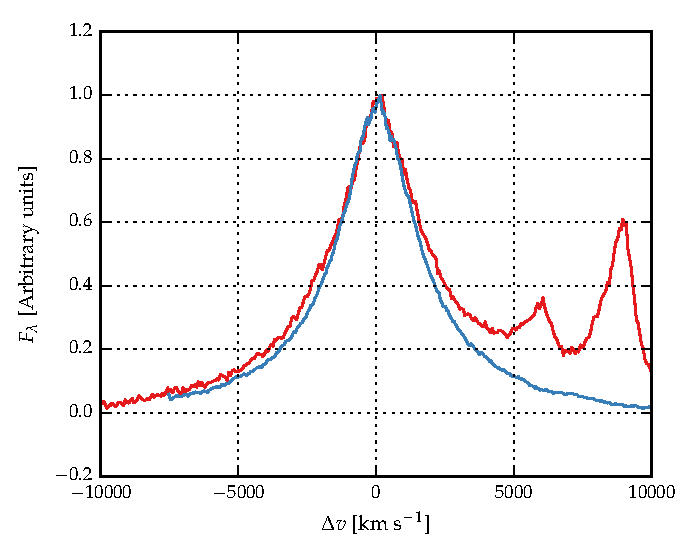
\includegraphics[width=0.8\linewidth]{figures/chapter03/ha_hb_composite.pdf} 
    \caption[{The \ha (blue) and \hb (red) emission line regions in the median composite spectrum, shown as function of the velocity shift from the respective predicted line peak wavelengths.}]{The \ha (blue) and \hb (red) emission line regions in the median composite spectrum, shown as function of the velocity shift from the respective predicted line peak wavelengths. The backgroud continuum and optical \ion{Fe}{II} emission has been modelled and subtracted. The line fluxes have been scaled in order for the profile shapes to be readily compared.}
    \label{fig:balmer_composite}
\end{figure}


\subsection{Measuring the quasar systemic redshift}
\label{sec:zsys}

An accurate measure of the quasar's systemic redshift is required in order for the blueshift of the \ion{C}{IV} emission line to be determined.
Balmer emission centroids are available for all quasars in the catalogue and so we use this to define the systemic redshift.

For 62 and 86 quasars in the \ha and \hb samples respectively narrow [\ion{O}{III}] emission is also detected with sufficient S/N to measure the line properties. 
In the model fit to the \hb region the velocity centroids of the broad \hbns-line and the core component of the [\ion{O}{III}] emission were deliberately determined separately.
We find the intrinsic difference in the velocity centroids of the \ha and \hb emission and the narrow [\ion{O}{III}] emission to have a dispersion of 300 and 400 \kms, which is very similar to the value found by \citet{shen16b}. 
However, the median velocity centroid of the narrow component of the [\ion{O}{III}] emission is blueshifted by 250\kms\, relative to the centroid of the broad Balmer line. 
Applying our parametric model fitting routine to the composite spectrum from \citet{hewett10}, which is constructed using relatively low redshift SDSS quasars with $L_{\mathrm Bol}\sim10^{44}$\,erg\,s$^{-1}$, the centroids of the broad component of \hb and the narrow component of [\ion{O}{III}] are found to be at essentially identical velocities, suggesting that the blueshifting of narrow [\ion{O}{III}] could be luminosity dependent.

As described in Section~\ref{sec:spec_measures}, the broad components of \ha and \hb were modelled with up to two Gaussians, with identical velocity centroids. 
If there is any significant asymmetry in these lines then the emission will be poorly fit by our model and the 
redshift derived from the peak of the best-fitting model could be biased. 
To investigate this possibility we relaxed the requirement for the centroids of the two broad Gaussians to be the same, and measured the systemic redshift from the peak of the composite profile. 
With this new, more flexible model, the mean absolute difference between the centroids of the two Gaussian components used to model \ha and \hb was 480 and 780 \kms respectively. 
With these adjustments, we found the mean difference between the [\ion{O}{III}]- and \hans(\hbns) based redshift estimates to be -100(-120) \kms and the scatter to be 290(320) \kms. 
Therefore, the shift between the Balmer and [\ion{O}{III}] velocities is reduced, suggesting that there might be a $\sim$100 \kms systematic bias in our measurements of the quasar systemic redshift.  
Regardless, since both the systematic offset and the scatter are small in comparison to the dynamic range in \ion{C}{IV} blueshifts, the blueshift-based empirical correction we will derive does not depend on whether the broad Balmer emission or the [\ion{O}{III}] centroid is used to define the systemic redshift, or how the broad Balmer emission is parameterized. 

Later, in section XX, we demonstrate how improvements in the estimation of systemic redshifts from ultraviolet quasar spectra means that it is now possible to quantify the distribution of \ion{C}{IV}-blueshifts in the observed population as a whole. 
Clearly, this is a crucial development in making a blueshift-based correction viable.

\subsection{Balmer/\ion{C}{IV} line widths as a function of \ion{C}{IV}-blueshift}
\label{sec:correction}

In this section we directly compare the \ion{C}{IV} and \hans/\hb line widths as a function of the \ion{C}{IV} blueshift. 
Because virial BH mass estimates are generally based on the \hb FWHM, we first convert our \ha FWHM measurements to equivalent \hb FWHM using Eq.~\ref{eq:ha2hb}.  
In Figs.~\ref{fig:correction_ha} and \ref{fig:correction_hb} we show the \ion{C}{IV} FWHM relative to both the (\hbns-scaled) \ha FWHM and the \hb FWHM, as a function of the \ion{C}{IV} blueshift. 

Employing the same Bayesian fitting framework described in Section~\ref{sec:hahbcomparison}, we fit independent linear models to the \ion{C}{IV} FWHM relative to the \ha and \hb FWHM as a function of the \ion{C}{IV} blueshift. 
As before, our model has an additional parameter representing any intrinsic scatter in the relationship between the variables which is independent of measurement errors.  
We also tested a model where some fraction of the data points (which is free to vary) are drawn from an outlier distribution, represented by a broad Gaussian centered on the mean of the data. 
We found, however, that the inferred outlier fraction was very low (0.004, corresponding to $\sim$0.7 data points) and so did not include such a component in our model. 

\begin{figure}
    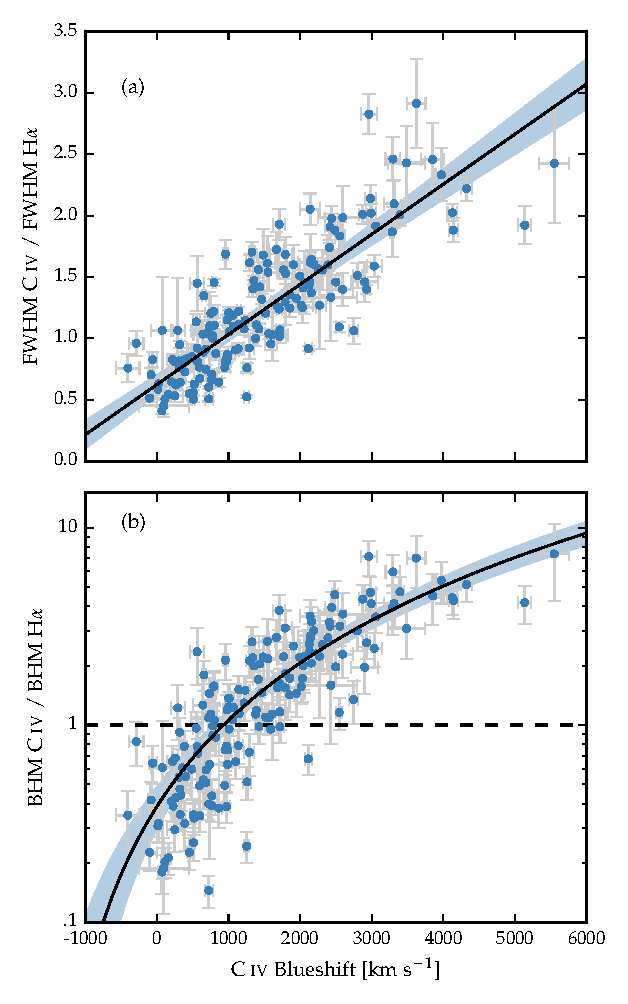
\includegraphics[width=\textwidth]{figures/chapter03/fwhm_and_bhm_ha.pdf} 
    \caption[{\ion{C}{IV} FWHM relative to \ha FWHM (a), and \ion{C}{IV} based BH mass (BHM) compared to \ha based mass (b), both as a function of the \ion{C}{IV} blueshift.}]{\ion{C}{IV} FWHM relative to \ha FWHM (a), and \ion{C}{IV} based BH mass (BHM) compared to \ha based mass (b), both as a function of the \ion{C}{IV} blueshift. The black line is our best-fit linear model, and the shaded region shows the 2-$\sigma$ uncertainties on the slope and intercept. The \ha FWHM have been scaled to match the \hb FWHM using Eq.~\ref{eq:ha2hb}.}  
    \label{fig:correction_ha}
\end{figure}

\begin{figure}
    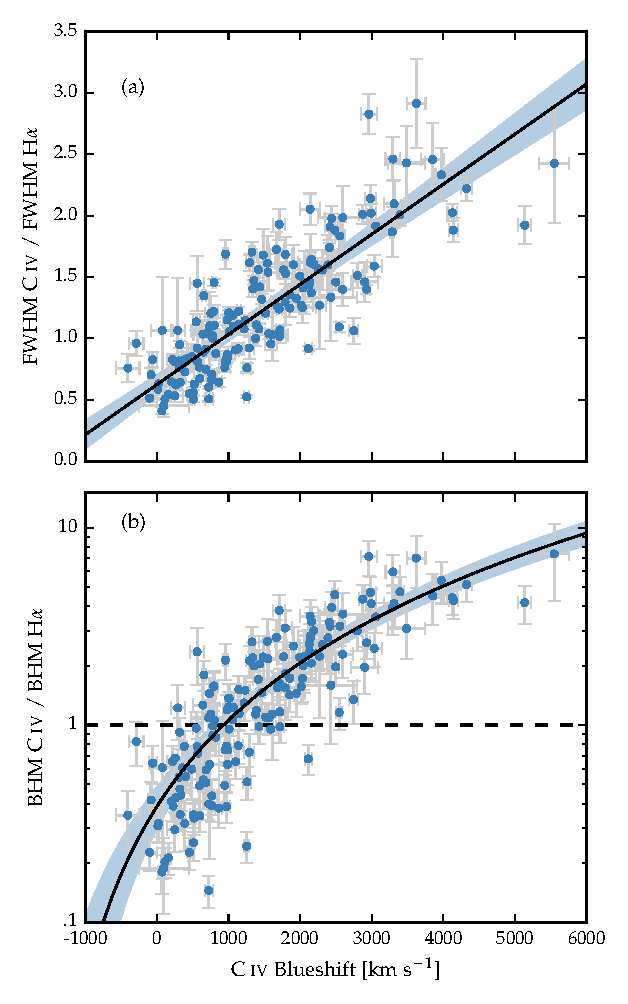
\includegraphics[width=\textwidth]{figures/chapter03/fwhm_and_bhm_ha.pdf} 
    \caption{\ion{C}{IV} FWHM relative to \hb FWHM (a), and \ion{C}{IV} based BH mass (BHM) compared to \hb based mass (b), both as a function of the \ion{C}{IV} blueshift.}  
    \label{fig:correction_hb}
\end{figure}

In Fig.~\ref{fig:mcmc_parameters} we show the one- and two-dimensional projections of the posterior distribution from the linear fit to the FWHM \ion{C}{IV}/\ha ratio. 
The projections from the FWHM \ion{C}{IV}/\hb fit, which we do not show, have very similar appearances.
In Fig.~\ref{fig:correction_ha} we plot the maximum likelihood model and the 2$\sigma$ uncertainties on the model parameters. 
The maximum likelihood line is given by  

\begin{equation}
    \label{eq:hafwhm}
    \mathrm{FWHM}(\mathrm{C}\,\textsc{iv}, \mathrm{Corr.}) = \frac{\mathrm{FWHM}(\mathrm{C}\,\textsc{iv}, \mathrm{Meas.})}{ (0.41\pm0.02) \left(\frac{\mathrm{C}\,\textsc{iv}\, Blueshift}{10^3 {\mathrm \,km\,s^{-1}}} \right) + (0.62\pm0.04)}
\end{equation}

\noindent for the \ion{C}{IV}/\ha fit and 

\begin{equation}
    \label{eq:hbfwhm}
    \mathrm{FWHM}(\mathrm{C}\,\textsc{iv}, \mathrm{Corr.}) = \frac{\mathrm{FWHM}(\mathrm{C}\,\textsc{iv}, \mathrm{Meas.})}{ (0.36\pm0.03) \left(\frac{\mathrm{C}\,\textsc{iv}\, Blueshift}{10^3 {\mathrm \,km\,s^{-1}}} \right) + (0.61\pm0.04)}
\end{equation}

\noindent for the \ion{C}{IV}/\hb fit. 
The intercepts of the two relations are consistent, while the difference between the slopes is only marginally inconsistent given the quoted uncertainties. 

The intrinsic scatter in the data about the linear relation we infer is $0.23 \pm 0.02$ and $0.25 \pm 0.02$ for the \ha and \hb fits respectively. 
The intrinsic scatter for the \ha fit is represented by the Normal probability density distribution shown in Fig.~\ref{fig:intrinsic_scatter}. 
In the same figure we show the distribution of the orthogonal displacement of each data point from the best-fitting linear relationship. 
The two distributions are well-matched, which demonstrates that our model is a good representation of the data and the measurement errors on the data points are small relative to the intrinsic scatter.    

The overall (intrinsic and measurement) scatter about the best-fitting model is slightly higher when the \ion{C}{IV} line-widths are compared to \hb (0.12 dex) than when compared to \ha (0.10 dex). 
This is likely due, at least in part, to the generally higher S/N of the \ha emission. 
In addition, contributions from the strong [\ion{O}{III}] doublet in the vicinity of \hb make de-blending the \hb emission more uncertain. 
As a consequence, for quasars where \ha and \hb are both measured, the mean uncertainty on the \ha FWHM is 130\kms, compared to 340\kms for \hbns. 

In the next section we use both the \ha and \hb lines to calculate unbiased BH masses. 
However, we use the \ha measurements to derive an empirical \ion{C}{IV} blueshift based correction to the \ion{C}{IV} masses (Eq.~\ref{eq:masscorrection}) because of the issues related to the accurate modelling of the \hbns-profile just described.  
An extra advantage, which is evident in Figs.~\ref{fig:correction_ha} and \ref{fig:correction_hb}, is that the \ha sample has a better \ion{C}{IV} blueshift coverage. 
However, as can be seen from the similarity of Equations \ref{eq:hafwhm} and \ref{eq:hbfwhm}, our results would not change significantly were we instead to use the \hb sample. 

\begin{figure}[h!]
    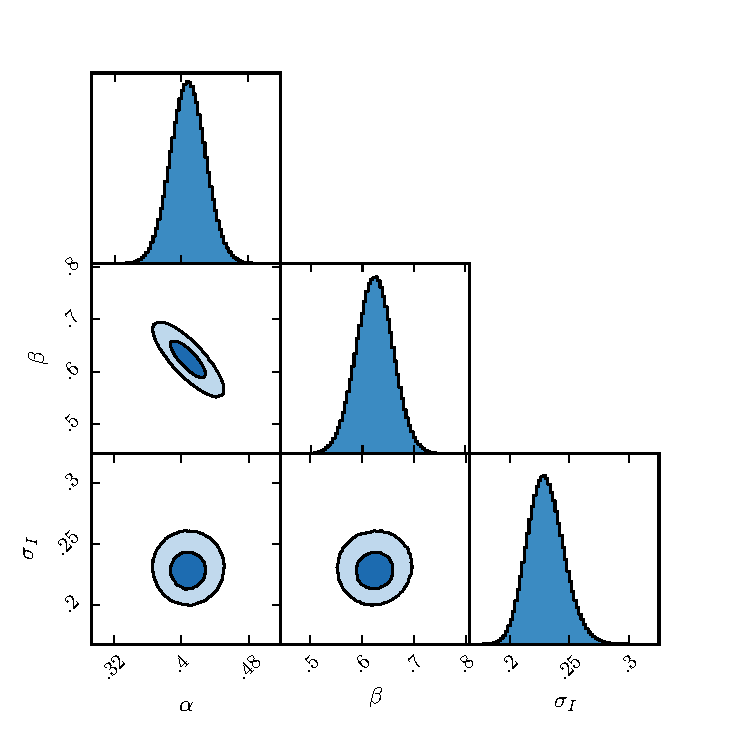
\includegraphics[width=\textwidth]{figures/chapter03/civ_ha_mcmc_parameters.pdf} 
    \caption[{One- and two-dimensional projections of the MCMC sample of the posterior distribution for a linear fit to the FWHM \ion{C}{IV}/\ha ratio as a function of the \ion{C}{IV} blueshift.}]{One- and two-dimensional projections of the MCMC sample of the posterior distribution for a linear fit to the FWHM \ion{C}{IV}/\ha ratio as a function of the \ion{C}{IV} blueshift. In the two-dimensional projections we show 1- and 2-$\sigma$ contours. The posterior distribution for the linear fit to the FWHM \ion{C}{IV}/\hb ratio, which we do not show, has a very similar appearance.} 
    \label{fig:mcmc_parameters}
\end{figure}

\begin{figure}[h!]
    \centering 
    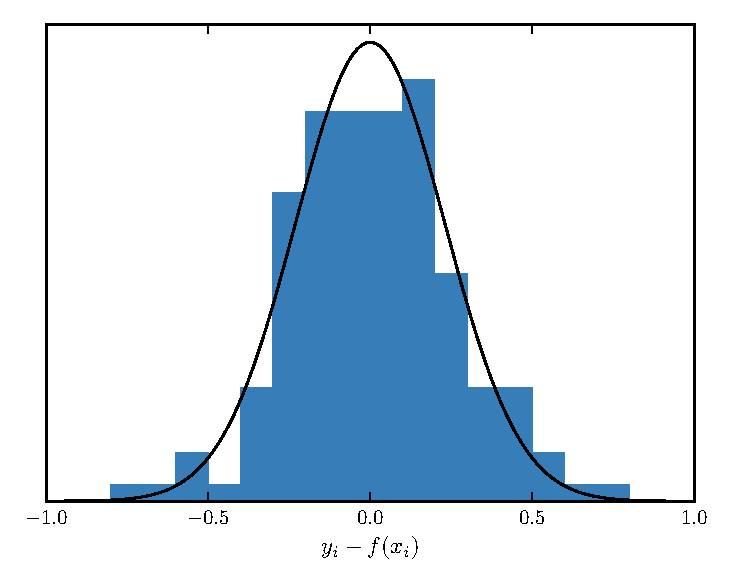
\includegraphics[width=0.7\textwidth]{figures/chapter03/intrinsic_scatter.pdf} 
    \caption[{The distribution of the orthogonal displacement of each data point from the best-fitting linear relationship in the fit to FWHM(\ion{C}{IV})/FWHM(\hans) as a function of the \ion{C}{IV} blueshift.}]{The distribution of the orthogonal displacement of each data point from the best-fitting linear relationship in the fit to FWHM(\ion{C}{IV})/FWHM(\hans) as a function of the \ion{C}{IV} blueshift (blue histogram). The black curve is a Normal distribution with a width equal to the intrinsic scatter in the population inferred from the fit. The two distributions are well-matched, which demonstrates that our model is a good representation of the data and the measurement errors on the data points are small relative to the intrinsic scatter.} 
    \label{fig:intrinsic_scatter}
\end{figure}

\subsection{\ion{C}{IV} based virial BH mass estimates}

Virial BH masses were calculated using the widely adopted \citet{vestergaard06} calibrations. 
The \citet{vestergaard06} \ion{C}{IV} FWHM calibration uses the monochromatic continuum luminosity at 1350\,\AA\, to predict the BLR radius and corresponds to ($a=6.66$, $b=2$, $c=0.53$) in Eq.~\ref{eq:virialmass}. 
For the \hb calibration, \citet{vestergaard06} use the monochromatic continuum luminosity at 5100\,\AA\, and calibration coefficients corresponding to ($a=6.91$, $b=2$, $c=0.5$).
BH masses are computed using the line and continuum properties given in Table~\ref{tab:bhm-specmeasure}, and we convert our \ha emission-line velocity-width measures to predicted \hb widths using Eq.~\ref{eq:ha2hb}.

In the lower panels of Figs.~\ref{fig:correction_ha} and \ref{fig:correction_hb} the \ion{C}{IV}-based estimates are compared to the \hans/\hb estimates as a function of the \ion{C}{IV} blueshift. 
There is a strong systematic error in the \ion{C}{IV}-based masses as a function of blueshift, which is a direct consequence of the FWHM trend described in the previous section. 
The \ion{C}{IV} emission-based BH-masses are in error by a factor of more than five at 3000\kms in \ion{C}{IV} emission blueshift and the overestimate of the BH-masses reaches a factor of 10 for quasars exhibiting the most extreme blueshifts, $\gtrsim$5000\kms. 

The virial product is the product of the virial velocity squared and the BLR radius \citep[e.g.][]{shen13}, and is proportional to the BH mass. 
We use the corrected \ion{C}{IV} FWHM given by Eq.~\ref{eq:hafwhm} as an indicator of the virial velocity, and adopt the same $R-L$ relation for the 1350\,\AA\, continuum luminosity as \citet{vestergaard06} (i.e. $R \propto L^{0.53}$). 
To find the constant scaling factor necessary to transform the virial product in to a BH mass we compute the inverse-variance weighted mean difference between the virial products and the \hans-based masses. 
The virial BH mass can then be expressed in terms of the corrected \ion{C}{IV} FWHM and monochromatic continuum luminosity at 1350\,\AA

\begin{equation}
  \label{eq:masscorrection}
  \mathrm{MBH}(\mathrm{C}\,\textsc{iv}, \mathrm{Corr.}) = 10^{6.71}\left( \frac{ \mathrm{FWHM}(\mathrm{C}\,\textsc{iv}, \mathrm{Corr.})}{10^3 \mathrm{\,km\,s^{-1}}} \right)^2 \left( \frac{\lambda \mathrm{L}_{\lambda} (1350 \text{\AA}) }{10^{44} \mathrm{\,erg\,s^{-1}}}  \right)^{0.53}
\end{equation}

Given measured \ion{C}{IV} emission line FWHM and blueshift, equations 4 and 6 can then be used to provide an unbiased estimate of the quasar BH mass.

\subsection{\ion{C}{IV}-derived BH masses at low \ion{C}{IV} blueshift}

\todo{Might work better later in discussion.}
In this section, we consider why the \ion{C}{IV} based masses of quasars with modest \ion{C}{IV} blueshifts ($\lesssim1000$\kms) are systematically underestimated relative to masses derived from the Balmer lines (Figs. \ref{fig:correction_ha} and \ref{fig:correction_hb}). 

Reverberation mapping measurements of nearby AGN have revealed the BLR to be stratified, with high-ionisation lines, including \ion{C}{IV}, emitted closer to the BH than low-ionisation lines, including \ha and \hb \citep[e.g.][]{onken02}.
\citet{vestergaard06} found that the \ion{C}{IV}-emitting region is at approximately half the radius of the \hbns/\ha emitting region.
Given the $\Delta V \propto R_{\mathrm BLR}^{-0.5}$ virial relation, this leads to the prediction that the \ion{C}{IV} line widths should be $\simeq 1.4$ times broader than \ha for a given BH mass. 
More recently, \citet{denney12} found that there is a significant contribution from gas at larger radii to the \ion{C}{IV} emission line, enhancing the profile at lower-velocity and leading to smaller FWHM or dispersion values. 
The ratio of the line widths is therefore predicted to be lower than the factor of $\simeq 1.4$. 

The \ha and \ion{C}{IV} FWHM of the 77 quasars with \ion{C}{IV} blueshifts $<$1200\,\kms\, are linearly correlated, as expected if the dynamics of the BLR clouds are dominated by virial motions. 
The median \ion{C}{IV}/\ha FWHM ratio is 0.97 with standard deviation 0.31. 
Thus, as predicted by considering the contribution from low-velocity gas at large radii, the FWHM-based comparison results in a systematically lower median \ion{C}{IV}/\hans.

As a direct consequence of the empirically small \ion{C}{IV}/\ha FWHM ratio, the \ion{C}{IV}-derived BH mass estimates are systematically lower than the corresponding \hans-derived masses when the blueshift is small.
This can be seen in Fig~\ref{fig:correction_ha}, where for almost every quasar with a \ion{C}{IV} blueshift $<$1200\,\kms, the \ion{C}{IV}-derived BH mass is smaller than the corresponding \hans-derived mass.
The median fractional difference between the two estimates is 0.60.  

\section{Practical application of the \ion{C}{IV}-based correction to virial BH-mass estimates}

\subsection{Recipe for unbiased \ion{C}{IV} based BH masses}
\label{sec:ch3-recipe}

\subsubsection{Measuring the systemic redshift}

Equations 4 and 6 together provide an un-biased estimate of the virial BH mass given the FWHM and blueshift of \ion{C}{IV}, together with the continuum luminosity at 1350\,\AA. 
The FWHM is readily obtained, either directly from the data, or, via the fitting of a parametric model to the \ion{C}{IV}-emission line. 
The blueshift -- defined as the bisector of the cumulative line flux -- is also straightforward to measure and our preferred procedure is described in Section~\ref{sec:civmeasure}.
The only potential complication arises in establishing the quasar systemic redshift and hence defining the zero-point for the \ion{C}{IV}-blueshift measurement, since both the blueshift and the systemic redshift cannot be determined from \ion{C}{IV} alone. 
In practice, when rest-frame optical lines are accessible, as is the case for the quasar sample here, an accurate systemic redshift can be obtained. 
The [\ion{O}{III}] doublet and the Balmer lines all have velocity centroids very close to systemic, and the same is true for the broad \ion{Mg}{II} doublet. 
For quasars at very high redshifts, $z\sim6$, systemic redshifts can also be derived using the [\ion{C}{II}] 158 $\mu$m emission in the sub-millimetre band \citep[e.g.][]{venemans16}. 
However, in general, for example in determining the BH-masses of quasars at redshifts $z>2$, if only the rest-frame ultraviolet region is available determining a reliable systemic redshift is non-trivial. 

The SDSS DR7 pipeline redshifts are not sufficiently reliable to measure the \ion{C}{IV} blueshift accurately because, in part, the \ion{C}{IV} emission line itself contributes to the determination of the quasar redshifts. 
This is demonstated in Fig.~\ref{fig:civ_space_z_compare}a, in which we plot the \ion{C}{IV}-blueshift versus \ion{C}{IV}-emission equivalent width (EW) using the SDSS pipeline redshifts and the blueshifts calculated by \citet{shen11}.  
A strong trend in the blueshift values as a function of line EW is not evident in Fig.~\ref{fig:civ_space_z_compare}a; structure in the parameter space is being masked because the \ion{C}{IV} emission line is itself being used in the determination of the quasar redshifts. 

\begin{figure}
    \centering 
    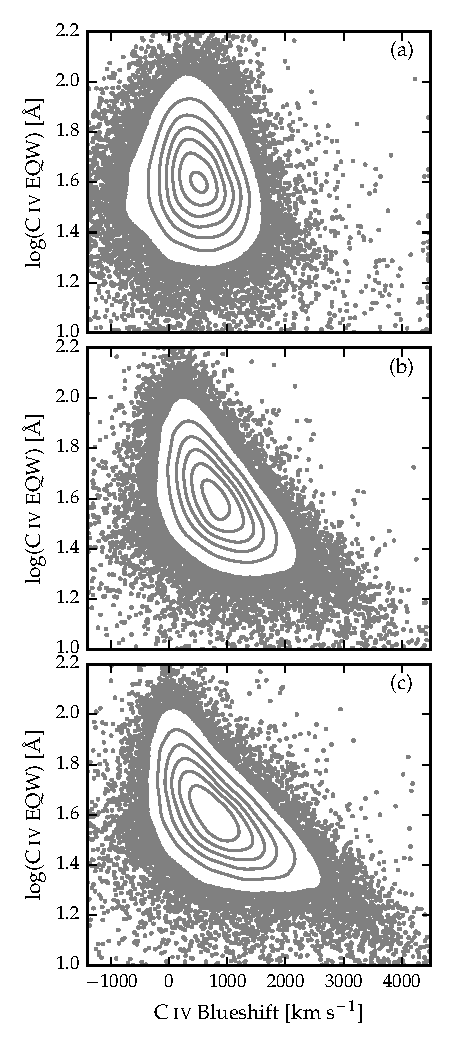
\includegraphics[width=8cm]{figures/chapter03/civ_space_z_compare.pdf}
    \caption[{Rest-frame EW versus blueshift of the broad \ion{C}{IV}-emission line for 32,157 SDSS DR7 quasars at $1.6 < z < 3.0$.}]{Rest-frame EW versus blueshift of the broad \ion{C}{IV}-emission line for 32,157 SDSS DR7 quasars at $1.6 < z < 3.0$. Panel (a) uses \ion{C}{IV} line parameters from \citet{shen11} and SDSS pipeline systemic redshifts. Panels (b) and (c) use systemic redshifts from \citet{hewett10} and Allen \& Hewett (2017, in preparation) respectively, and \ion{C}{IV} line measurements described in Sec.~\ref{sec:civmeasure}. In regions of high point-density, contours show equally-spaced lines of constant probability density generated using a Gaussian kernel-density estimator.} 
    \label{fig:civ_space_z_compare}
\end{figure}

The redshift-determination scheme of \citet{hewett10} provided much improved redshifts, not least because the redshift estimates for the majority of quasars were derived using emission-lines other than the \ion{C}{IV}-line itself. 
Figure \ref{fig:civ_space_z_compare}b shows SDSS DR7 quasars in the same \ion{C}{IV} parameter space as Figure \ref{fig:civ_space_z_compare}a, but now using \citet{hewett10} redshifts. 
The improved redshift estimates are predominantly responsible for the differences seen in Fig.~\ref{fig:civ_space_z_compare}a and b; the appearance in Fig.~\ref{fig:civ_space_z_compare}b of the extension to high blueshift for quasars with low \ion{C}{IV} EW is particularly evident.

\citet{shen16b} and our own work shows that there is an intrinsic variation of $\sigma$$\simeq$220\kms in the velocity centroids of the broad-line region relative to a systemic-frame defined by the quasar narrow-line regions.
The redshifts for quasars in the SDSS DR10 and DR12 catalogues \citep{paris14,paris17} possess errors of $\simeq$500-750\kms \citep{paris12, font-ribera13}. The impact of low spectrum S/N for fainter quasars in all the SDSS data releases increases the uncertainty further. 
Table~\ref{tab:bhm_error} includes the values for the fractional error in the corrected BH-mass that result from a given error in the determination of the systemic rest-frame. 
For example, the fractional error in the corrected BH mass is 0.39 for a quasar with a 1000\kms\, \ion{C}{IV} blueshift when there is a 500\kms\, uncertainty in the quasar systemic redshift.   

\begin{table}
  \centering
  \caption{The fractional error on the corrected BH mass as a function of \ion{C}{IV} blueshift for different uncertainties in the quasar systemic redshift.}
  \label{tab:bhm_error}
  \centering
    \begin{tabular}{ccccc} 
    \hline
    \multirow{1}{*}{} & \multicolumn{4}{c}{\ion{C}{IV} blueshift (\kms) } \\
    \multicolumn{1}{c}{$\delta$v (\kms)} & 
    \multicolumn{1}{c}{0} &
    \multicolumn{1}{c}{1000} &
    \multicolumn{1}{c}{2000} &
    \multicolumn{1}{c}{4000}  \\
    \hline
    250 & 0.33 &  0.20 &  0.14 & 0.09 \\
    500 & 0.65 & 0.39 & 0.28 & 0.18 \\
    1000 &1.30 & 0.79 & 0.57 & 0.36 \\
    \hline
    \end{tabular}
\end{table}

Of potentially more significance for studies of BH-masses as a function of quasar and host-galaxy properties are redshift errors that depend on the form of the quasar ultraviolet SED.
The large systematic variation in the \ion{C}{IV} emission-line profile within the population is evident from figures 11 and 12 of \citet{richards11}. 
The plots and analysis in \citet{richards11} employ the quasar redshifts from \citet{hewett10} but, as is evident from the figures, the systematic variation in the \ion{C}{IV} shape is correlated with changes in the quasar SEDs, including the strengths of the \ion{Si}{III}$\lambda$1892 and \ion{C}{III}$\lambda$1908 emission lines in the rest-frame ultraviolet. 
As a consequence, the redshifts from \citet{hewett10} still suffer from systematic errors that are correlated with the shape, and particularly the blueshift, of the \ion{C}{IV} emission line.
For the \citet{hewett10} redshifts, and ultraviolet emission-line based redshifts in general, quasars with large \ion{C}{IV} EW and modest blueshifts have relatively small ($\simeq$300\kms) SED-dependent redshift errors.
Redshift uncertainties as large as $\simeq$1000\kms for such quasars are unusual and the large relative error in the corrected \ion{C}{IV} BH-mass given in Table~\ref{tab:bhm_error} is pessimistic. 

Conversely, systematic redshift errors are greatest for quasars with large blueshifts, reaching $\sim$750\kms in the extreme for the \citet{hewett10} values. 
The associated error in the corrected \ion{C}{IV} BH-masses is, however, mitigated somewhat due to the smaller gradient of the MBH(\ion{C}{IV})/MBH(Balmer) relation at large \ion{C}{IV} blueshift (see Figs.~\ref{fig:correction_ha} and \ref{fig:correction_hb}). 
A definitive quantification of any systematic SED-dependent errors present in the quasar redshifts contained in the SDSS DR12 catalogue is not yet available but the principal component analysis (PCA) based redshift estimates are expected to be largely free of SED-dependent systematics. 

Using published redshift estimates, notably those from \citet{hewett10} for the SDSS DR7 quasars and the BOSS PCA-based redshifts from \citet{paris17} for SDSS DR12, the correction formula given in Section~\ref{sec:correction} produces significant improvements to \ion{C}{IV}-based BH mass estimates.
In a forthcoming work, Allen \& Hewett (in preparation) will present a new redshift-estimation algorithm that produces redshifts independent of the \ion{C}{IV} blueshift and other variations in the ultraviolet SEDs of luminous quasars.
The low-ionization emission lines visible in the rest-frame ultraviolet (over wavelengths from \ion{Mg}{II}$\lambda\lambda$2796,2803 down to the \ion{O}{I}$\lambda$1304+\ion{Si}{II}$\lambda$1307 blend) using the new redshift-algorithm are located at rest-frame wavelengths in excellent agreement with the systemic redshift defined using the rest-frame narrow-line optical \ion{O}{III} doublet and broad-line \hb and \hans.
SED-dependent systematic errors are below the apparent inherent dispersion of $\simeq220$\kms associated with broad emission line redshifts \citep{shen16b}.

Figure~\ref{fig:civ_space_z_compare}c shows the \ion{C}{IV} emission line parameters calculated using the Allen \& Hewett redshift-estimation algorithm.  
The systematic trends seen in Fig.~\ref{fig:civ_space_z_compare}b, in particular the extension to high blueshift at low \ion{C}{IV} EW, become more apparent in Fig.~\ref{fig:civ_space_z_compare}c, as expected from consideration of the known SED-related errors in the redshifts from \citet{hewett10}.
A population of quasars with only modest blueshifts and low EW is also apparently still present. 

\subsubsection{\ion{C}{IV} emission line blueshift measurements}
\label{sec:civmeasure}

The differences in the distribution of \ion{C}{IV} emission line properties seen in the three panels of Fig.~\ref{fig:civ_space_z_compare} are due primarily to the change in the systemic redshift estimates. 
It is also necessary, however, to obtain a measure of the \ion{C}{IV} emission line `location' in order to calculate the blueshifts. 
When working with moderately-sized samples, parametric fits to the emission-line profile may be undertaken using careful mask-definition to minimise the effect of absorption features on the profiles used for the parametrization, and this is the approach we followed in Section~\ref{sec:spec_measures}.

Effective analysis of the tens of thousands of spectra from SDSS DR7, and now DR12, however, requires a more robust scheme to determine a \ion{C}{IV}-blueshift estimate that is not very sensitive to the range of S/N among the spectra or the presence of narrow absorption systems within the \ion{C}{IV}-emission profile. 
\citet{shen11} provide a discussion (their section~3) of the factors that effect the measurement of broad emission lines in quasar spectra of modest S/N. 
Their careful analysis of the \ion{C}{IV} emission properties employed the results of parametric fits of three Gaussians to the spectra. 
Our own experiments in quantifying the \ion{C}{IV} emission properties of SDSS spectra showed that a simple non-parametric measure of the \ion{C}{IV} emission location reduced the number of outliers significantly. 
Visual inspection of spectra demonstrated that the improvement is due primarily to the identification of, and interpolation over, associated and outflow absorption systems, which forms part of the non-parametric measurement scheme. 

We therefore chose to use a non-parametric scheme to measure the blueshift of the \ion{C}{IV{}} line, which we will now describe. 
A continuum is first defined as a power-law of wavelength, $f(\lambda) \propto \lambda^{-\alpha}$, with the slope, $\alpha$, determined using the median\footnote{The median is used to improve the robustness of the continuum estimate from the relatively small wavelength intervals.} values of the flux in two continuum windows at 1445--1465 and 1700--1705\AA\, (the same wavelengths as adopted by \citet{shen11}). 
The \ion{C}{IV} emission line is taken to lie within the wavelength interval 1500-1600\AA, a recipe that is commonly adopted \citep[e.g.][]{shen11, denney13}. 
To reduce the impact of narrow absorption systems on the emission-line profile a `pseudo continuum' is defined by applying a 41-pixel median filter to the quasar spectrum.
Pixels within the \ion{C}{IV} profile that lie more than 2$\sigma$ below the pseudo-continuum are deemed to be affected by absorption and added to an `absorber'-mask. 
Two pixels on either side of each such pixel are also included in the mask. 
For each masked pixel, the flux values in the spectrum are replaced by values from the pseudo-continuum. 
The wavelength that bisects the cumulative total line flux is recorded and the blueshift is defined in exactly the same way as in Section~\ref{sec:spec_measures}. 

Allen \& Hewett will publish improved redshifts for all quasars in the SDSS DR7 and DR12 catalgoues. 
At the same time we will publish catalogues of unbiased BH masses for both SDSS DR7 and DR12 based on the Allen \& Hewett redshifts. 
The components from the mean-field independent component analysis \citep[see][for an application to astronomical spectra]{allen13} used in the Allen \& Hewett redshift algorithm will also be published.
With these components, if a rest-frame ultraviolet spectrum is available, it will be straightforward to determine the systemic redshift, via a simple optimisation procedure, and hence calculate the \ion{C}{IV} blueshift. 

\subsection{Systematic trends in residuals}

The scatter about the best-fitting line in the \ion{C}{IV}/\ha FWHM versus \ion{C}{IV}-blueshift relation is $\sim$0.1 dex, an order of magnitude smaller than the size of the \ion{C}{IV}-blueshift dependent systematic but, nevertheless, still significant.
With a view to reducing the scatter further, we searched for measurable parameters which correlate with the scatter at fixed \ion{C}{IV} blueshift, including the luminosity, redshift, [\ion{O}{III}] equivalent width (EW), and \ion{Fe}{II} EW.
The only significant correlation we find is with the \ha FWHM (Fig.~\ref{fig:residuals_ha_fwhm}).
Quasars with broad \ha lines tend to lie below the relation while quasars with narrow \ha tend to lie above it.
One possibility is that this correlation is simply due to random scatter (either intrinsic or measurement error) in the \ha FWHM which, with the other quasar properties fixed, would naturally produce a correlation between FWHM(\ion{C}{IV})/FWHM(\hans) and FWHM(\hans).
However, the fact that we see no such correlation between the model residuals and the \ion{C}{IV} FWHM suggests that the \ha FWHM correlation could be revealing somthing more fundamental. 
The \hans/\hb FWHM is part of `eigenvector 1' (EV1), the first eigenvector in a principal component analysis which originated from the work of \citet{boroson92}.    
While a number of parameters have been considered within the EV1 context \citep[e.g.][]{brotherton99},
Fig.~\ref{fig:residuals_ha_fwhm} suggests that part of the scatter between the Balmer and \ion{C}{IV} velocity widths might be attributed to differences in the spectral properties which are correlated with EV1 \citep{marziani13}. 

The shape of the line can be characterised by the ratio \citep[FWHM/$\sigma$, where $\sigma$ is the dispersion, derived from the second moment velocity; e.g.][]{kollatschny11,Kollatschny13}. 
FWHM/$\sigma$ $\simeq 2.35$ for a Gaussian profile, while FWHM/$\sigma$ $\simeq 1$ for a peakier Lorentzian profile\footnote{Strictly FWHM/$\sigma$ $\rightarrow 0$ for a Lorentzian profile, but values close to unity are typical when the dispersion is calculated over a velocity range, $\simeq\pm10\,000$\kms, used to parametrize broad emission lines in quasar spectra.}.
In our sample, we find the residuals and the \ha FWHM correlate with the shape of the line.   
\todo{I think I mentioned this earlier so okay to delete there.}
The narrow lines are, on average, `peakier' (with FWHM/$\sigma\simeq$ 1) than the broader lines (with FWHM/$\sigma\simeq$ 2).   
The origin of the Balmer-line shape correlation is not clear but one possibility is an orientation-dependence of the \ha FWHM \citep[e.g.][]{shen14}. 
In this scenario quasars with broader emission lines are more likely to be in an edge-on orientation relative to our line of sight.  
    
At radio wavelengths, the morphology of the radio structure, parametrized in terms of `core dominance' is believed, at least in a statistical sense, to be a proxy for the orientation of the accretion disk \citep[e.g.][]{jackson91}.
Twenty core- quasars and six lobe-dominated quasars were identified in our sample, but no statistically significant differences in the \ha line-widths of the two samples were found. 
It should be noted that the sub-sample of radio-detected quasars is small and the effectiveness of the test is further compromised by the lack of radio-detected quasars at large blueshifts \citep[see figure 14 of][for example]{richards11}.

\todoinline{Maybe include: On the other hand, a concern is raised by the observation that the BLR structure changes with emission-line FWHM (Kollatschny \& Zetzl 2011). They show that FWHM/$\sigma$ is a strong, smooth
function of FWHM. These changes in line profile shapes suggest that the balance between rotation, random velocities, and in- or outflow changes with line width. Hints of this were seen in earlier work (Collin et al.
2006; Marziani \& Sulentic 2012).} 

There are currently very few reverberation-mapping measurements of quasars with large \ion{C}{IV} blueshifts.
Looking to the future, the results of the large on-going statistical reverberation mapping projects \citep[e.g.][]{shen15,kingoz15} for luminous quasars at high-redshift will shed new light on the Balmer line emitting region of the BLR for quasars with a range of \ion{C}{IV} blueshifts and lead to a greater understanding of the relation between the Balmer line profile and the BH mass. 

\begin{figure}
    \centering 
    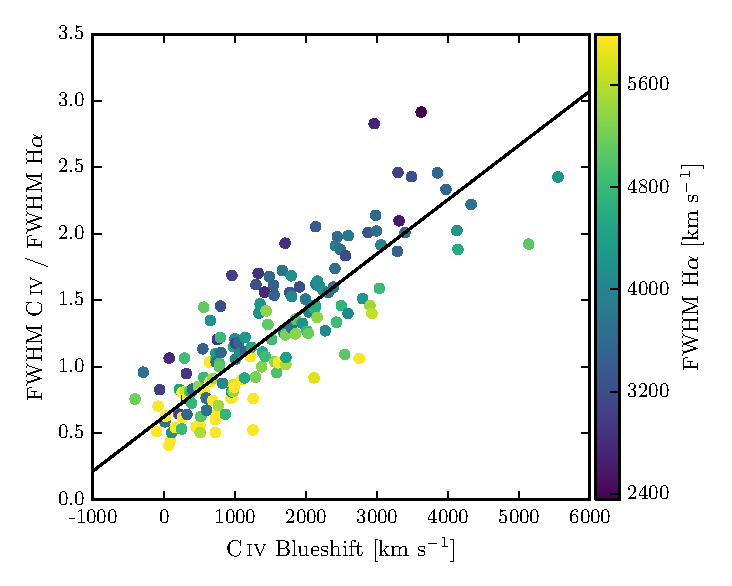
\includegraphics[width=0.8\textwidth]{figures/chapter03/fwhm_correction_color.pdf}  
    \caption[{Same as Fig.~\ref{fig:correction_ha}a, with the marker colour representing the \ha FWHM.}]{Same as Fig.~\ref{fig:correction_ha}a, with the marker colour representing the \ha FWHM. At fixed \ion{C}{IV} blueshift, there is a clear \ha FWHM dependent systematic in the model residuals.}   
    \label{fig:residuals_ha_fwhm}
\end{figure}

\subsection{Effectiveness of the \ion{C}{IV} blueshift based correction to BH masses}
\label{sec:effectiveness}

\begin{figure}
    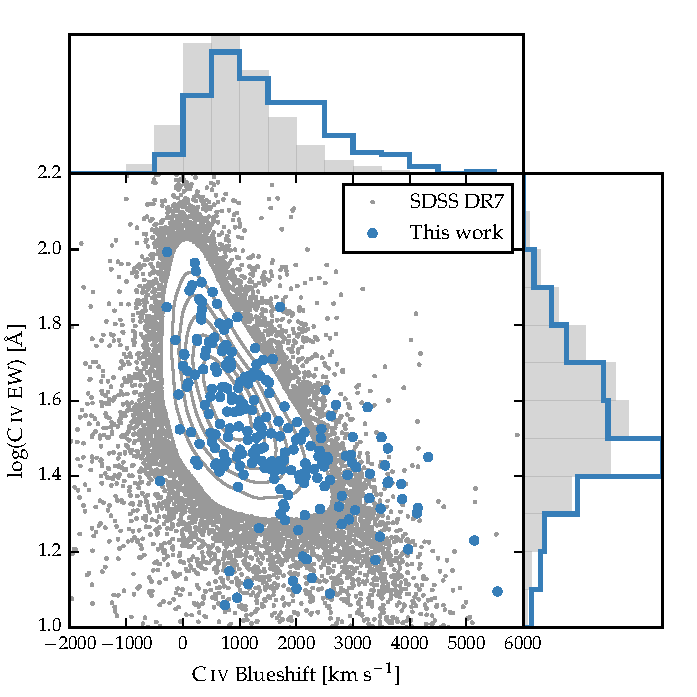
\includegraphics[width=\columnwidth]{figures/chapter03/civ_space.pdf} 
    \caption[{Rest-frame EW versus blueshift of the broad \ion{C}{IV}-emission line for 32,157 SDSS DR7 quasars at $1.6 < z < 3.0$ and our sample.}]{Rest-frame EW versus blueshift of the broad \ion{C}{IV}-emission line for 32,157 SDSS DR7 quasars at $1.6 < z < 3.0$ ({\it grey}) and our sample ({\it blue}). For the SDSS quasars, the systemic redshifts used to calculate the blueshifts are from \citet{hewett10} and \ion{C}{IV} emission properties are decribed in Paper I. In regions of high point-density, contours show equally-spaced lines of constant probability density generated using a Gaussian kernel-density estimator. Our sample has very good coverage; the shift to high blueshifts is a result of the high luminosity of our sample in relation to the SDSS sample and the correlation between luminosity and blueshift.} 
    \label{fig:civ_space}
\end{figure}

Figure~\ref{fig:civ_space} demonstrates that our sample has an excellent coverage of the EW-blueshift parameter space in relation to SDSS DR7 quasars at redshifts $1.6 < z < 3.0$. 
The systematic offset to higher \ion{C}{IV} blueshifts for our catalogue relative to the SDSS quasars as a whole is a result of the higher mean luminosity relative to the SDSS sample (Fig.~\ref{fig:lzplane}).
Our sample includes 21 quasars with \ion{C}{IV} blueshifts $>$3000\kms, and extends to $\sim$5000\kms, i.e. at the very extreme of what is observed in this redshift and luminosity range. 
Our investigation thus demonstrates that the \ion{C}{IV}-blueshift based correction derived in this chapter is applicable to very high blueshifts. 
Conversely, there are no quasars in our catalogue with \ion{C}{IV} blueshifts $\lesssim$0\kms and we caution against extrapolating the correction formula to negative blueshifts. 

\begin{figure}
    \centering 
    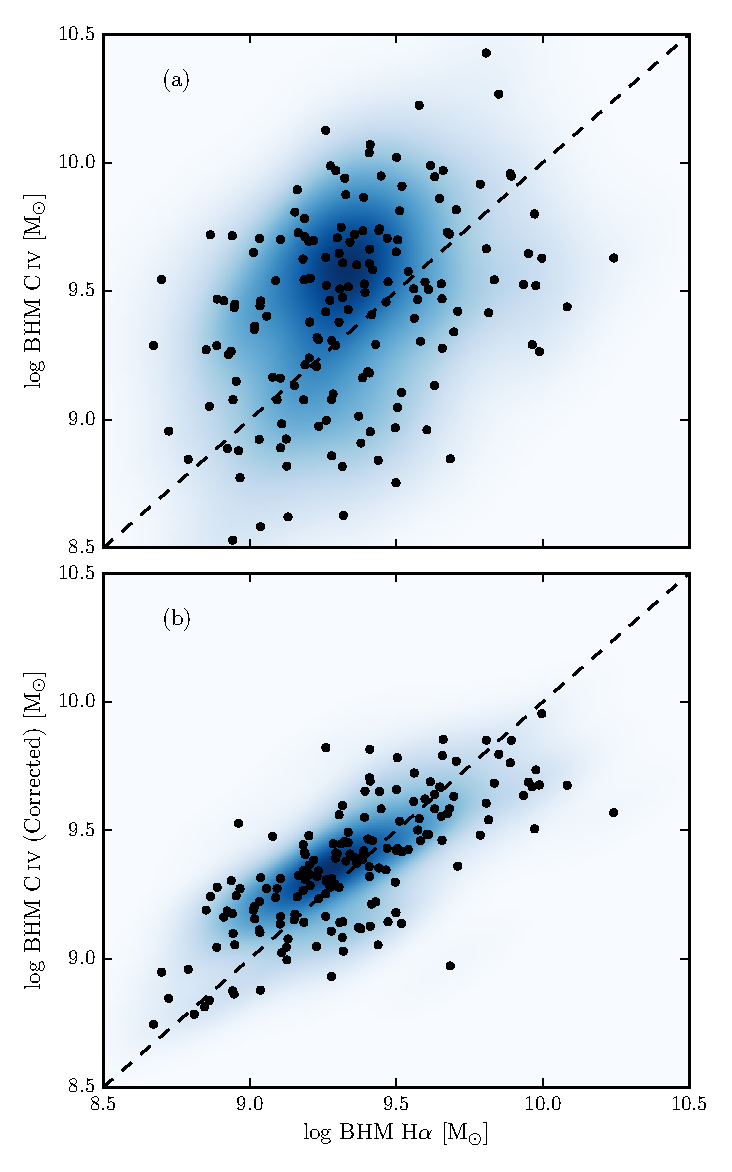
\includegraphics[width=0.8\columnwidth]{figures/chapter03/bhm_comparison.pdf} 
    \caption[{Comparison of the \ion{C}{IV}- and \hans-based BH masses before and after applying the \ion{C}{IV} blueshift-based correction to the \ion{C}{IV} FWHM.}]{Comparison of the \ion{C}{IV}- and \hans-based BH masses before (a) and after (b) applying the \ion{C}{IV} blueshift-based correction to the \ion{C}{IV} FWHM. The density of the plotted points (estimated using a Gaussian kernel density estimator) is represented by the colour. The correction to the \ion{C}{IV} BH masses decreases the scatter by from 0.4 to 0.2 dex. \todoinline{Should definitely include some empirical validation of ICA redshifts since that is what we are telling people to use.}}   
    \label{fig:bhm_comparison}
\end{figure}

Figure~\ref{fig:bhm_comparison} compares the \ion{C}{IV}- and \hans-based BH masses before and after applying the blueshift-based correction to the \ion{C}{IV} FWHM.
Before the correction, the correlation between the \ion{C}{IV}- and \hans-based BH masses is very weak, and the scatter between the masses is 0.4 dex. 
After correcting the \ion{C}{IV} FWHM for the non-virial contribution, the correlation improves dramatically. 
The scatter between the corrected \ion{C}{IV}-based masses and the \hans-based masses is reduced to 0.2 dex. 
The scatter is 0.24 dex at low \ion{C}{IV} blueshifts ($\sim$0\kms) and 0.10 dex at high blueshifts ($\sim$3000\kms). 

\begin{figure}
    \centering 
    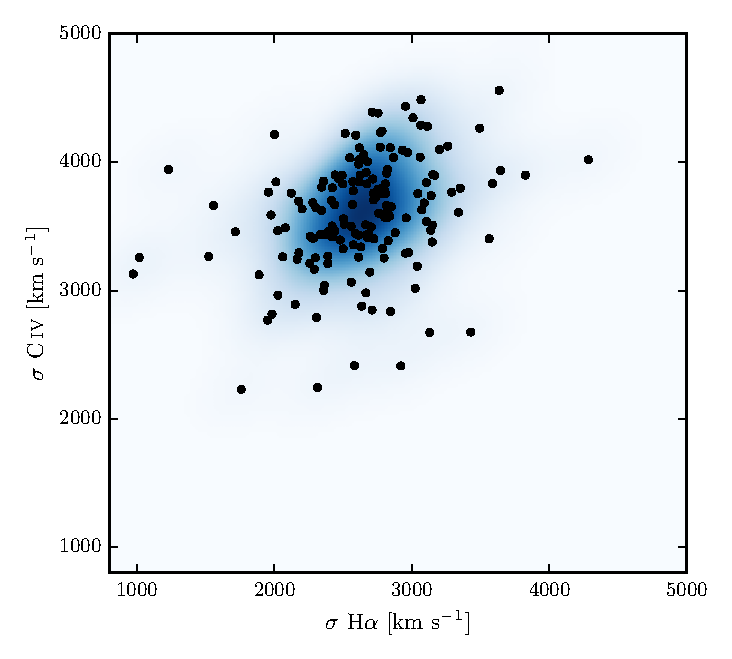
\includegraphics[width=0.8\columnwidth]{figures/chapter03/dispersion_comparison.pdf} 
    \caption[{Comparison of the \ion{C}{IV} and \ha line dispersion, $\sigma$.}]{Comparison of the \ion{C}{IV} and \ha line dispersion, $\sigma$. The density of the plotted points (estimated using a Gaussian kernel density estimator) is represented by the colour. Estimating a reliable BH mass from the \ion{C}{IV} FWHM and blueshift line is substantially more effective than using the \ion{C}{IV} line dispersion with, or without, the line blueshift. The \ion{C}{IV} dispersion values are larger than the corresponding \ha measurements by a factor of 1.4 on average, which is consistent with reverberation mapping measurements \citep{vestergaard06}.} 
    \label{fig:dispersion_comparison}
\end{figure}

There has been a considerable amount of attention regarding the relative merits of using the FWHM or dispersion to characterise the velocity width \citep[e.g.][]{denney13}.
The existence of a trend in the \ion{C}{IV}-dispersion values with \ion{C}{IV} blueshift is evident from inspection of the bottom left panel of Fig.~\ref{fig:line_comparison_civ} but the systematic trend relative to the spread at fixed blueshift is significantly smaller than when using \ion{C}{IV} FWHM. 
Therefore, without the blueshift information, using the line dispersion would yield a more accurate BH mass than the FWHM (Fig.~\ref{fig:dispersion_comparison}). 

The correlation between the \ha and \ion{C}{IV} line dispersion is, however, weak. 
The Pearson coefficient for the correlation is 0.36 (and just 0.15 when the \hb measurements are used in place of \hans). 
Furthermore, there is little dynamic range in the line dispersion: the scatter is just 480 and 460\kms for \ha and \ion{C}{IV} respectively. 
The observation suggests that the line dispersion does not fully trace the dynamic range in BH mass present in the quasar population. 
At least part of the reason is that the line dispersion is difficult to measure reliably in current survey-quality data, particularly because of the sensitivity to flux ascribed to the wings of the emission line \citep[e.g.][]{mejia-restrepo16}.
Figures~\ref{fig:bhm_comparison} and \ref{fig:dispersion_comparison} demonstrate that estimating a reliable BH mass from the \ion{C}{IV} FWHM and blueshift line is substantially more effective than using the \ion{C}{IV} line dispersion with, or without, the line blueshift. 

\subsection{Comparison to previous prescriptions}

\begin{figure*}
    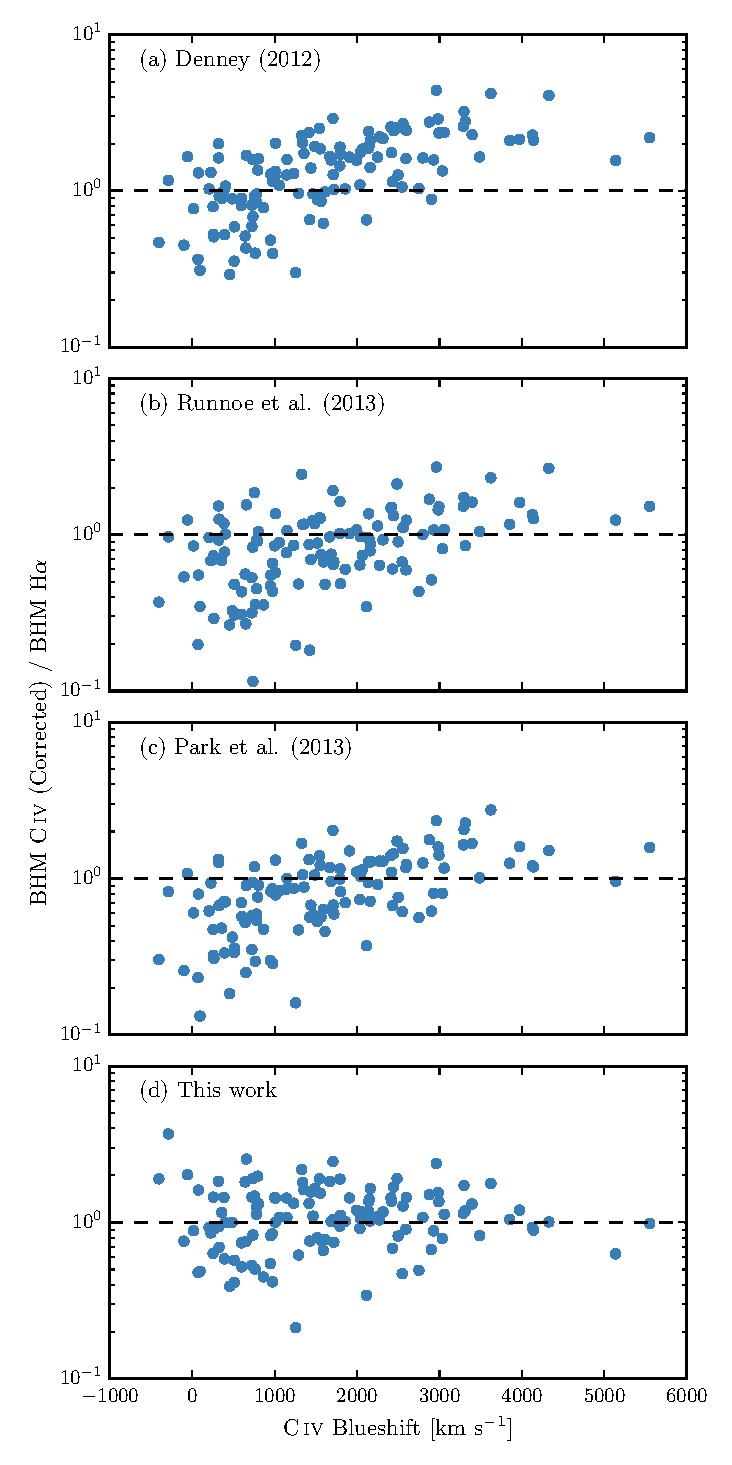
\includegraphics[width=0.9\textwidth]{figures/chapter03/corrections.pdf}  
    \caption[{Comparison of BH mass estimates derived from \ion{C}{IV} and \ha as a function of the \ion{C}{IV} blueshift.}]{Comparison of BH mass estimates derived from \ion{C}{IV} and \ha as a function of the \ion{C}{IV} blueshift. Corrections to the \ion{C}{IV}-based masses have been applied based on the shape (FWHM/$\sigma$) of the \ion{C}{IV} emission line \citep[a;][]{denney12}, the peak flux ratio of the \ion{Si}{IV}+\ion{O}{IV} blend relative to \ion{C}{IV} \citep[b;][]{runnoe13}, by significantly reducing the dependence of the derived BH mass on the \ion{C}{IV} velocity-width \citep[c;][]{park13}, and based on the \ion{C}{IV} blueshift (d; this chapter).}
    \label{fig:compare_corrections}
\end{figure*}

In Fig.~\ref{fig:compare_corrections} we compare the \ion{C}{IV} blueshift-based correction presented in this chapter to various prescriptions which have been proposed in the literature to derive BH masses from the \ion{C}{IV} line which are consistent with the masses derived from the Balmer lines. 
In each case we compare the corrected \ion{C}{IV}-based masses to the \hans-based masses as a function of the \ion{C}{IV} blueshift. 
The correction proposed by \citet{runnoe13} is based on the spectral region at rest-frame wavelengths of $\sim$1400\,\AA \ (see below). 
Therefore, our analysis is based on the 123 quasars with spectra covering this region. 

In Fig~\ref{fig:compare_corrections}a the \ion{C}{IV} BH masses have been corrected using the \ion{C}{IV} shape (FWHM/$\sigma$) based correction proposed by \citet{denney12}. 
\citet{denney12} found the level of contamination in single-epoch spectra from non-reverberating gas to be correlated with the shape (FWHM/$\sigma$) of the \ion{C}{IV} profile. 
In our sample, we observe a strong correlation between the shape of the \ion{C}{IV} line and its blueshift (Fig.~\ref{fig:line_comparison_civ}); between the two extremes in the \ion{C}{IV} blueshift distribution the line shape changes from FWHM/$\sigma\sim$1 to 2.5. 
The investigation of \citet{denney12} was based on a sample of reverberation mapped quasars, which have a narrow range of \ion{C}{IV}-emission line shapes, including the absence of any objects with large \ion{C}{IV} blueshifts. 
The correction is not applicable at large \ion{C}{IV} blueshifts. 
Therefore, while the consistency between the \hans- and \ion{C}{IV}-based masses at low \ion{C}{IV} blueshifts is improved, at high \ion{C}{IV} blueshifts the \ion{C}{IV}-based masses remain seriously overestimated.

As explained above, reliably measuring the quasar systemic redshift from the UV region of the spectrum has proved difficult. 
However, the situation is improved dramatically by the new scheme developed by Allen \& Hewett (2017, in preparation). 
Given the difficulty of measuring reliable \ion{C}{IV} blueshifts without the Allen \& Hewett scheme, \citet{runnoe13} opted instead to use the continuum-subtracted peak flux ratio of the ultraviolet emission-line blend of \ion{Si}{IV}+\ion{O}{IV} (at 1400\,\AA) to that of \ion{C}{IV} to correct for non-virial contributions to the \ion{C}{IV} velocity width. 
This parameter was chosen because it showed the strongest correlation with the FWHM \ion{C}{IV}/\hb residuals, as well as with the strengths of optical \ion{O}{III} and \ion{Fe}{II}. 

Following \citet{runnoe13}, we measure the peak flux by fitting a model with four Gaussian components (two for each emission line) to the continuum-subtracted flux.
As is evident from Fig.~\ref{fig:civ_space}, a correlation exists between the blueshift and equivalent width of \ion{C}{IV}: \ion{C}{IV} emission which is strongly blueshifted is typically weak. 
The \ion{Si}{IV}+\ion{O}{IV} emission-line blend, however, shows significantly less systematic variation. 
Therefore, the \ion{Si}{IV}+\ion{O}{IV}-based correction is quite effective in practice: the systematic bias in the \ion{C}{IV} BH masses at large \ion{C}{IV} blueshifts is reduced to a factor of $\sim2$ (Fig.~\ref{fig:compare_corrections}b).
However, the \ion{C}{IV} based masses are still systematically overestimated at large \ion{C}{IV} blueshifts. 

In contrast to the widely-used \citet{vestergaard06} \ion{C}{IV}-based virial BH mass calibration, the more recent \citet{park13} calibration significantly reduces the dependence of the derived masses on the emission-line velocity width (from the $V^2$ dependence predicted assuming a virialized BLR to just $V^{0.56}$).
As a consequence, the \ion{C}{IV} based masses of the quasars with large \ion{C}{IV} blueshifts are much reduced (Fig.~\ref{fig:compare_corrections}c).
However, the systematic error in the \ion{C}{IV}-based BH masses as a function of \ion{C}{IV} blueshift remains. 

As a comparison, the \ion{C}{IV}-based masses shown in Fig~\ref{fig:compare_corrections}d have been corrected using to the \ion{C}{IV} blueshift-based procedure presented in this chapter. 
No systematic in the BH masses as a function of the \ion{C}{IV} blueshift is evident. 

\section{Population trends with \ion{C}{IV} blueshift}
\label{sec:hatrends}

\begin{figure}
    \centering 
    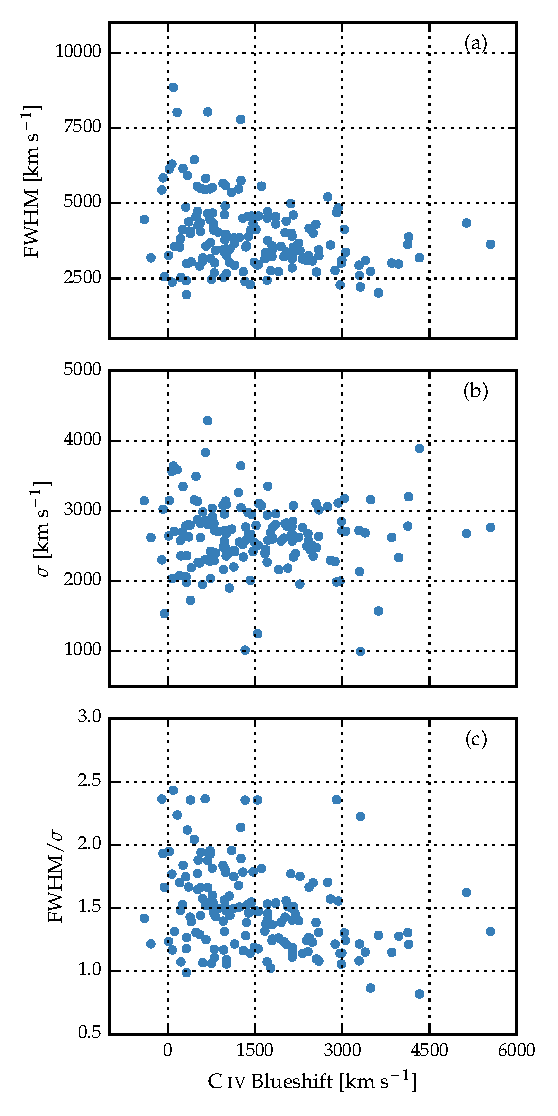
\includegraphics[width=0.8\linewidth]{figures/chapter03/ha_comparisons_paper2.pdf} 
    \caption{The FWHM, dispersion ($\sigma$) and shape (FWHM/$\sigma$) of \ha as a function of the \ion{C}{IV} blueshift.}
    \label{fig:line_comparison_ha}
\end{figure} 

% \begin{figure}
%     \centering 
%     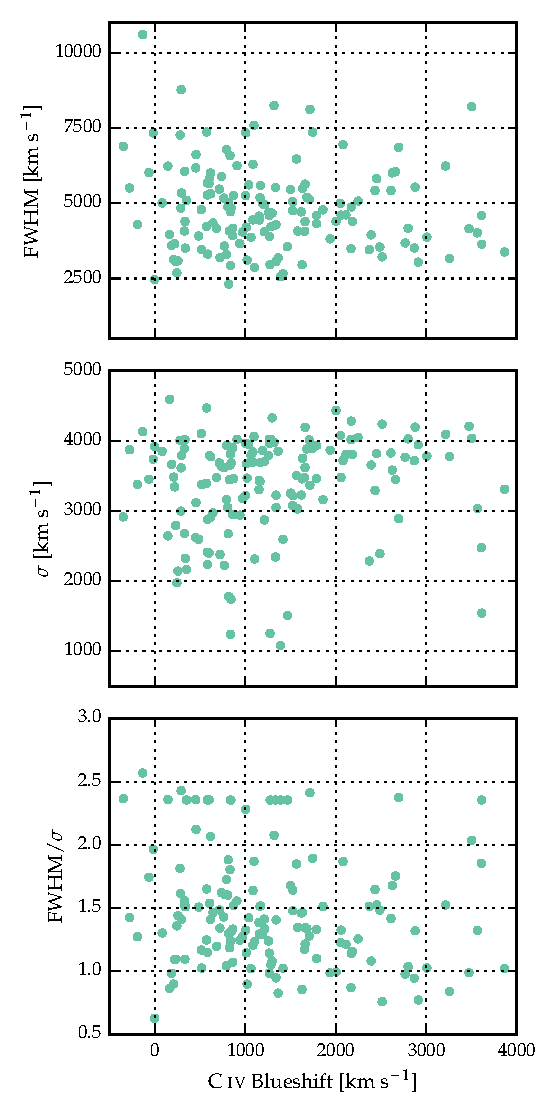
\includegraphics[width=0.8\linewidth]{figures/chapter03/hb_comparisons_paper2.pdf} 
%     \caption{The FWHM, dispersion ($\sigma$) and shape (FWHM/$\sigma$) of \hb as a function of the \ion{C}{IV} blueshift.}
%     \label{fig:line_comparison_ha}
% \end{figure} 

\begin{figure}
    \centering
    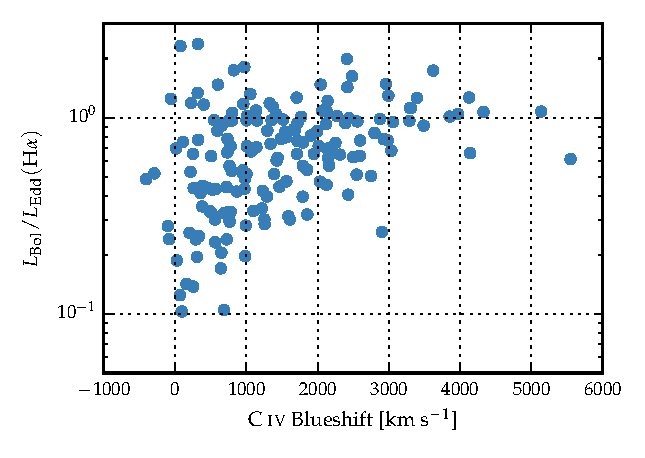
\includegraphics[width=0.8\linewidth]{figures/chapter03/ha_edd_civ_bs.pdf}
    \caption[{\hans-derived Eddington ratio versus \ion{C}{IV} blueshift.}]{\hans-derived Eddington ratio versus \ion{C}{IV} blueshift. At blueshift $\gtrsim$ 2000\kms\, all quasars have high accretion rates ($L/L_{\mathrm Edd} \simeq 1$). This is in agreement with \citet{kratzer15}, but in contrast to what one would derive from naive use of \ion{C}{IV}-based BH mass scaling relations.}
    \label{fig:ha_edd_civ_bs}
\end{figure}

As shown in Fig.~\ref{fig:line_comparison_ha}, there are systematic variations in the \ha line profile as a function of the \ion{C}{IV} blueshift. 
At \ion{C}{IV}-blueshift $<$1200\,\kms, the \ha FWHM range is $\simeq2000 - 8900$\,\kms, with mean $\simeq$4300\,\kms.
However, amongst the quasars with \ion{C}{IV}-blueshift $>$2000\,\kms, the mean \ha FWHM=3500\,\kms, with a scatter of just 700\,\kms. 
The apparent trend of peakier \hans-emission, with FWHM/$\sigma$ close to unity, at large \ion{C}{IV}-blueshift is enhanced by the modest increase in \ha EW with blueshift. 
Amongst the low-\ion{C}{IV}-blueshift population there are in addition quasars with broader and more Gaussian-like \ha line profiles, with FWHM/$\sigma \simeq 2$ . 

The change in the \ha emission-line profiles as a function of \ion{C}{IV}-blueshift means that the \hans-FWHM derived BH masses at high-blueshift are smaller than the sample mean. 
We transformed the observed luminosity into a mass-normalised accretion rate (Eddington ratio).
To convert the monochromatic luminosity, which is observed, in to a bolometric luminosity we use the bolometric correction factor given by \citet{richards06} ($L_{\mathrm bol} = 9.26L_{5100}$).
Although there is evidence that the bolometric correction factor is a function of the luminosity, as well as of other parameters including the \ion{C}{IV} blueshift \citep{krawczyk13}, the differences are small over the parameter range covered by our sample, and for simplicity we adopt a constant factor. 

The results, shown in Fig.~\ref{fig:ha_edd_civ_bs}, demonstrate that at large blueshifts quasars are accreting at around their Eddington limits (Fig.~\ref{fig:ha_edd_civ_bs}). 
This finding is in accord with our interpretation that the blueshifting of \ion{C}{IV} is evidence for strong outflows resulting from the presence of a radiation-driven accretion-disc wind. 
\citet{richards02} found that quasars with large \ion{C}{IV} blueshifts have weak \ion{He}{II}.
This is evidence for weak soft X-ray continuum emission \citep{leighly04}, which would allow a strong line-driven wind to form.  
The strength of such a wind is predicted to be related to the quasar far-ultraviolet SED, which, in turn, could be related to the mass-accretion rate.

All of the objects in our sample which exhibit large \ion{C}{IV} blueshifts would be classified as population A in the \citet{sulentic00b} scheme based on the \ha FWHM. 
Our results therefore support the idea of the \citet{sulentic00b} A/B division being driven by the Eddington ratio, with population A sources possessing higher accretion rates.
However, we also observe a number of quasars which have high Eddington ratios but do not have line profiles suggestive of strong outflows in the \ion{C}{IV} BLR.  
This suggests that a high accretion rate is a necessary but not sufficient condition for the existence of outflows \citep{baskin05}. 

The two-dimensional nature of the \ion{C}{IV} emission line parametrization and the apparent anti-correlation between \ion{C}{IV} EW and \ion{C}{IV} blueshift suggests that the quasar population exhibits a continuum of properties. 
As such, more accurate \ion{C}{IV} blueshift measurements for SDSS-quasars should allow an improved mapping between the \ion{C}{IV}-emission properties and key physical parameters of the quasars.
This includes improving our understanding of the origin of quasars with exceptionally weak, blueshifted \ion{C}{IV} emission \citep[weak emission line quasars;][]{luo15} which could be exotic versions of wind-dominated quasars \citep{plotkin15}.

\subsection{Systematic biases in Balmer-based masses}

The interpretation described in the preceding section requires some caution since the emission-line shape (characterized by the value of FWHM/$\sigma$) of \ha is also changing as a function of the \ion{C}{IV} blueshift (Fig.~\ref{fig:line_comparison_ha}). 
At low \ion{C}{IV} blueshifts there are a range of shapes, but all of the quasars exhibiting large \ion{C}{IV} blueshifts have peaky \ha profiles with FWHM/$\sigma \simeq 1$. 
This raises the question of whether the \ha FWHM is a reliable proxy for the virial-induced velocity dispersion for the full range of \ha line shapes we have in our sample. 

\todo{Can move most of this to earlier section on residuals and then refer back to that.}
When calibrating the virial-product to masses derived independently using the BH mass \---\ stellar velocity dispersion ($M_\odot-\sigma$) relation, \citet{collin06} find that the scaling factor, $f$, is a factor $\sim2$ larger for their Population `1' sources (with FWHM/$\sigma < 2.35$ and essentially equivalent to population A of Sulentic and co-workers and to the high-blueshift quasars here) than for their Population 2 (with FWHM/$\sigma > 2.35$). 
For single-epoch BH-mass estimates, assuming a constant value of $f$, as is normally done \citep[e.g.][]{vestergaard06}, means that Population 1 masses will be underestimated and Population 2 will be overestimated.
In the context of this result from \citet{collin06}, our high-blueshift objects all possess peaky \hans-lines and, while our quasar sample probes much higher luminosities and masses, the true BH-masses may also be underestimated.
Adopting such an interpretation, the amplitude of the trend seen in Figs.~\ref{fig:correction_ha} and \ref{fig:correction_hb} might not be so pronounced.

As mentioned in Section~\ref{ch:intro} and discussed in \citet{richards11}, quasars with current reverberation mapping measurements have a restricted range of \ion{C}{IV}-line shapes. 
There are currently very few reverberation-mapping measurements of quasars with large \ion{C}{IV} blueshifts but the results of the large on-going statistical reverberation mapping projects \citep[e.g.][]{shen15} for luminous quasars at high-redshift will go some way to establishing whether the quasar broad line regions producing Balmer emission look the same for objects with very different \ion{C}{IV}-emission blueshifts. 

Although the EV1-trends \citep{sulentic00b,shen14} are most likely driven by the accretion rate, orientation may also have a role to play in determining the observed properties of the BLR. 
\citet{shen14} argue that a large part of the scatter observed in the \hb FWHM relates not to a spread in BH masses, but rather to the orientation of the BLR relative to the line-of-sight.
For this to be true, the BLR would need to be in a flattened disc-like geometry, in which case the observed line width would increase with the inclination of the disc relative to the line of sight. 
\citet{brotherton15b} found that the core-dominance of radio-loud quasars, which is believed to be a reliable proxy for orientation, at least in a statistical sense, is significantly correlated with the \hb FWHM and hence with the BH-mass estimates. 
This raises the question of whether the narrow \ha emission lines observed in the quasars with the largest \ion{C}{IV} blueshifts could be an orientation effect. 
However, there is no evidence that the \ion{C}{IV} blueshift is dependent on the orientation \citep[inferred from the radio core-dominance;][]{richards11,runnoe14}. 
Furthermore, \citet{leighly04} showed that the \ion{He}{II}\l1640 emission-line properties of quasars with large \ion{C}{IV} blueshifts are more consistent with differences in the SED rather than differences in the orientation.
\citet{collin06} showed that orientation effects were also sub-dominant to the Eddington ratio in determining the shape of the \hb line and
the \ha line shape trend we observe is consistent with the finding of \citet{marziani03} that the \hb emission profiles of high/low Eddington ratio low-$z$ quasars and type 1 Seyfert nuclei are well fit by Lorentzian and double Gaussian profiles respectively.  
Overall, therefore, orientation does not appear to be the dominant effect in determining the \ion{C}{IV} blueshift and correlated changes in the \ha line profile. 

\subsection{The BAL parent population}

Classical high-ionization BAL (HiBAL) quasars are also predominantly Population A objects in the scheme of \citet{sulentic00b}. 
\todo{Do I actually say BALs are removed from sample?}
There are no HiBAL quasars in our sample by design but it is generally accepted that quasars which show high-ionisation BALs are likely to be radiating with relatively high $L/L_{\mathrm Edd}$ \citep[e.g.][]{zhang14}. 
We therefore propose that the subset of the quasar population that exhibits large \ion{C}{IV}-emission blueshifts, with high-EW and narrow-\ha emission lines, may be directly related to the HiBAL quasar population \---\ perhaps even the `parent' population \citep{richards06conf}. 
A prediction of such a linkage is that near-infrared observations of the rest-frame optical spectra of HiBAL quasars will show strong, relatively narrow, Balmer emission lines, very similar to those of the quasars with high \ion{C}{IV}-blueshifts presented in this chapter \citep[see][for such a study]{runnoe13b}. 
\todo{I must have a few BALs. Make a composite spectra of Balmer lines of BALs?}

\subsection{The frequency of quasars with high accretion rates}

Quantifying the frequency of quasars producing outflows as a function of key parameters, e.g. quasar luminosity, BH-mass, redshift,... will be important to constrain models of quasar-galaxy evolution.  
At fixed BH mass, the intrinsic and the observed fraction of quasars exhibiting properties that depend on the Eddington ratio can differ significantly. 
As an illustration, we consider the implications for the intrinsic fraction of quasars possessing large \ion{C}{IV} blueshifts given the observed numbers in the $m_i<19.1$ flux-limited sub-sample of the SDSS DR7 quasar catalogue. 
In order to estimate the size of the selection effect, we considered the detection probability for a much-simplified quasar population. 
We assume that all quasars with \ion{C}{IV} blueshifts $>$1200\,\kms have enhanced accretion rates relative to the `normal' population (with \ion{C}{IV} blueshifts $<$1200\,\kms). 
If the accretion rate of the high-blueshift population is double the rate of the low-blueshift population (which is true in an average sense \---\ see Fig.~\ref{fig:ha_edd_civ_bs}), then the high-blueshift population will be brighter by $\simeq$0.75 magnitude.
Under the assumption that the BH mass distribution is independent of the \ion{C}{IV} blueshift, the high-blueshift population will then be over-represented in a flux-limited sample.
To estimate the size of the bias, we need to know how many more quasars, at redshifts $2 < z < 2.5$, there are with $m_i<19.1+0.75=19.85$ relative to $m_i < 19.1$.
This is the fraction of the population which, as a consequence of having enhanced accretion rates, are boosted above the survey flux limit.    
The main colour-selected SDSS DR7 quasar catalogue extends only to $m_i= 19.1$ and, assuming the luminosity function is continuous\footnote{The luminosity function and number-counts vary only smoothly \citep[e.g.][]{ross13} for the magnitude and redshift range used here.} we thus use the number counts at $m_i < 19.1$ and $m_i < 18.35$, which differ by a factor of $\simeq 4$. 

At redshifts $2 < z <2.5$, there are 3,834 quasars with \ion{C}{IV} blueshifts $<$1200\,\kms and 2,484 with blueshifts $>$1200\,\kms in the SDSS DR7 $m_i < 19.1$ quasar sample, a ratio of $\sim$2:1. 
The above calculation, although much idealised, suggests that the intrinsic fraction of high-blueshift quasars is a factor of four smaller than in the flux-limited sample (i.e. $\sim$15\,per cent of the ultraviolet-selected non-BAL quasar population). 

\section{Conclusions}
\label{sec:conclusions}

The main results of this chapter are as follows: 

\begin{itemize}
\item We have analysed the spectra of 230 high-luminosity ($10^{45.5}-10^{48}$\,\ergs), redshift $1.5 < z < 4.0$ quasars for which spectra of the Balmer emission lines and the \ion{C}{IV} emission line exist.
The large number of quasars in our spectroscopic catalogue and the wide range in \ion{C}{IV} blueshifts the quasars possess has allowed us to directly investigate biases in \ion{C}{IV}-based BH mass estimates which stem from non-virial contributions to the \ion{C}{IV} emission as a function of the \ion{C}{IV} blueshift, which, in turn, depends directly on the form of the quasar ultraviolet SEDs \citep{richards11}.
\item The \ion{C}{IV} emission-based BH-masses are systematically in error by a factor of more than five at 3000\kms in \ion{C}{IV} emission blueshift and the overestimate of the BH-masses reaches a factor of 10 for quasars exhibiting the most extreme blueshifts, $\gtrsim$5000\kms. 
\item We have derived an empirical correction formula for BH-mass estimates based on the \ion{C}{IV} emission line FWHM and blueshift.
The correction may be applied using equations 4 and 6 in Section~\ref{sec:correction}.
The large SED-dependent systematic error in \ion{C}{IV}-based BH-masses is removed using the correction formulae.
The remaining scatter between the corrected \ion{C}{IV}-based masses and the \hans-based masses is 0.24 dex at low \ion{C}{IV} blueshifts ($\sim$0\kms) and 0.10 dex at high blueshifts ($\sim$3000\kms). 
This is a significant improvement on the 0.40 dex scatter observed between the un-corrected \ion{C}{IV} and \ha BH masses. 
The correction depends only on the \ion{C}{IV} line properties - i.e. the FWHM and blueshift - and allows single-epoch virial BH mass estimates to be made from optical spectra, such as those provided by the SDSS, out to redshifts exceeding $z\sim 5$. 
\end{itemize}

\section{Future work}

\begin{itemize}
\item Clustering
\item Data-driven mapping
\end{itemize}

\section{Description of catalogue}

\begin{itemize}
    
  \item[2] Unique ID: QSOXXX.

  \item[] LogMBH\_Ha, LogMBH\_Ha\_Err

  \item[] Edd\_Ratio\_Ha, Edd\_Ratio\_Ha\_Err

  \item[] LogMBH\_Hb, LogMBH\_Hb\_Err

  \item[] Edd\_Ratio\_Hb, Edd\_Ratio\_Hb\_Err

  \item[] LogMBH\_CIV\_VP06, LogMBH\_CIV\_VP06\_Err

  \item[] Edd\_Ratio\_CIV\_VP06, Edd\_Ratio\_CIV\_VP06\_Err

  \item[] Add corrected BH mass 

  \item[] FWHM\_Broad\_Ha, FWHM\_Broad\_Ha\_Err

  \item[] Sigma\_Broad\_Ha, Sigma\_Broad\_Ha\_Err

  \item[] EQW\_Broad\_Ha, EQW\_Broad\_Ha\_Err

  \item[] LogL\_Broad\_Ha, LogL\_Broad\_Ha\_Err

  \item[] FWHM\_Broad\_Hb, FWHM\_Broad\_Hb\_Err

  \item[] Sigma\_Broad\_Hb, Sigma\_Broad\_Hb\_Err

  \item[] EQW\_Broad\_Hb, EQW\_Broad\_Hb\_Err
 
  \item[] LogL\_Broad\_Hb, LogL\_Broad\_Hb\_Err

  \item[] z\_Broad\_Ha. Repeated in chapter 4 with slightly different model.

  \item[] z\_Broad\_Hb. Repeated in chapter 4 with slightly different model. 

  \item[] WARN\_Ha (Remove 2, just flag 1 as low S/N)

  \item[] RedChi\_Ha

  \item[] WARN\_Hb (Remove 2, just flag 1 as low S/N)

  \item[] RedChi\_Hb

  \item[] FWHM\_CIV\_BEST, FWHM\_CIV\_BEST\_Err (remove best, make sure it's clear where it comes from) (Just give BEST values then note of which optical spectrum was used). 

  \item[] Sigma\_CIV\_BEST, Sigma\_CIV\_BEST\_Err

  \item[] Median\_CIV\_BEST, Median\_CIV\_BEST\_Err

  \item[] EQW\_CIV\_BEST, EQW\_CIV\_BEST\_Err

  \item[] LogL\_CIV\_BEST, LogL\_CIV\_BEST\_Err

  \item[] Max\_CIV\_BEST, Max\_CIV\_BEST\_Err   

  \item[] Max\_1400\_BEST, Max\_1400\_BEST\_Err

  \item[] 1400\_CIV\_BEST, 1400\_CIV\_BEST\_ERR

  \item[] RedChi\_CIV\_BEST

  \item[] WARN\_CIV\_BEST (will have removed warn=2, so should just be warn=1 low S/N flag)

  \item[] WARN\_1400\_BEST (remove 1400 max if warn=2)

  \item[] Blueshift\_CIV\_Ha, Blueshift\_CIV\_Ha\_Err

  \item[] Blueshift\_CIV\_Hb, Blueshift\_CIV\_Hb\_Err




\end{itemize}

